\chapter{In-depth Contrastive Error Analysis}
\label{chap:analysis}

% Length
% Graph factors
% Linguistic factors

% Peking: Ensemble method, combination of transition-based and graph-based
% Turku: Support Vector Machines
% Lisbon: A graph algorithm

In this chapter we present an in-depth contrastive error analysis of the results of SemEval-2015 for the Peking, Turku and Lisbon system submissions described in Chapter \ref{chap:semantic}. There where 6 submissions to SemEval-2015, including an `in-official' submission by a sub-set of the task organizers. We have made the choice of focusing on three of these parsing systems in our analysis. This is based on three criteria:

\begin{enumerate}
    \item The chosen systems should have the highest overall accuracy scores in SemEval-2015.
    \item The technical approach of the three parsing systems should differ from one another: both the local transition-based and global graph-based models that we introduced in Chapter \ref{chap:background} should be represented.
    \item When choosing between submissions where similar technical approaches are employed, we should exclude the system with the overall lowest accuracy score.
\end{enumerate}

The aim of our in-depth contrastive error analysis is to gain insights into the accuracy of state-of-the-art semantic dependency parsing. The study is performed in order to:

\begin{enumerate}
    \item Find similarities and differences in the results among a chosen set of parsing systems.
    \item Compare and contrast their strengths and weaknesses.
    \item Empirically identify and verify which types of errors that can be the focus of future research on improving the accuracy of semantic dependency parsing.
    \item Examine the possibility of using the results of our study to modify and improve upon an existing system, or create a new system, in order to push the envelope on the accuracy of the results presented in this chapter.
\end{enumerate}

% We will argue that the analysis presented in this chapter can highlight the correlation between the specific types of errors that these parsers make and their theoretical foundation. The analysis presented is thus based on the general knowledge of the parsing systems, as described in Chapter \ref{chap:semantic}, and the specific observations made in our analysis of their results from SemEval-2015.

In our analysis we draw inspiration from three similar studies by \citeA{McD:Niv:07}, \citeA{McD:Niv:11}, and \citeA{Choi:Tetreaul:Stent:15}. In these studies a comparative analysis of a set of syntactic parsers is presented, and various types of errors that these parsers produce are highlighted. The first and second study focus on three types of errors: (1) length factors, (2) graph factors, and (3) linguistic factors. The third study, in addition to these three factors, also examine the time complexity of parsing systems: where both training and parsing time is taken into consideration. We will structure our analysis in a similar fashion, but exclude time complexity, and include the multi-classification task of frame predication introduced in SemEval-2015. Our focus will thus be on four factors: (1) length factors, (2) graph factors, (3) linguistic factors, and (4) frames.

In addition to narrowing down the scope in terms of choosing three parsing systems, we also exclude results for the PAS target representation. The reasoning behind this is that the DM and PAS target representations are relatively similar. Examining Table \ref{fig:data} in Chapter \ref{chap:semantic}, we observe that DM and PAS are close to identical in the number of labels, percentage of graphs being trees, and percentage of dependencies being projective. The major difference between the two target representations is the percentage of so-called singletons, i.e. nodes not connected to any other node in the dependency graph. The DM target representation has approximately 5 times as many singletons as PAS. With the exception of singletons, we assume that our analysis of the DM results will yield similar results as PAS. This hypothesis was confirmed by running the error analysis on the PAS target representation, and observing that for most types of errors there is a strong correlation in the types of errors made when using the DM target representation for training and testing.

Before embarking on our in-depth contrastive error analysis, we will first recap and further examine some overall statistics on the three parsing systems that we will use as basis for our study.

\section{Overall Accuracy}

\begin{figure}[h]
    \centering
    \begin{minipage}{0.8\textwidth}
        \centering
        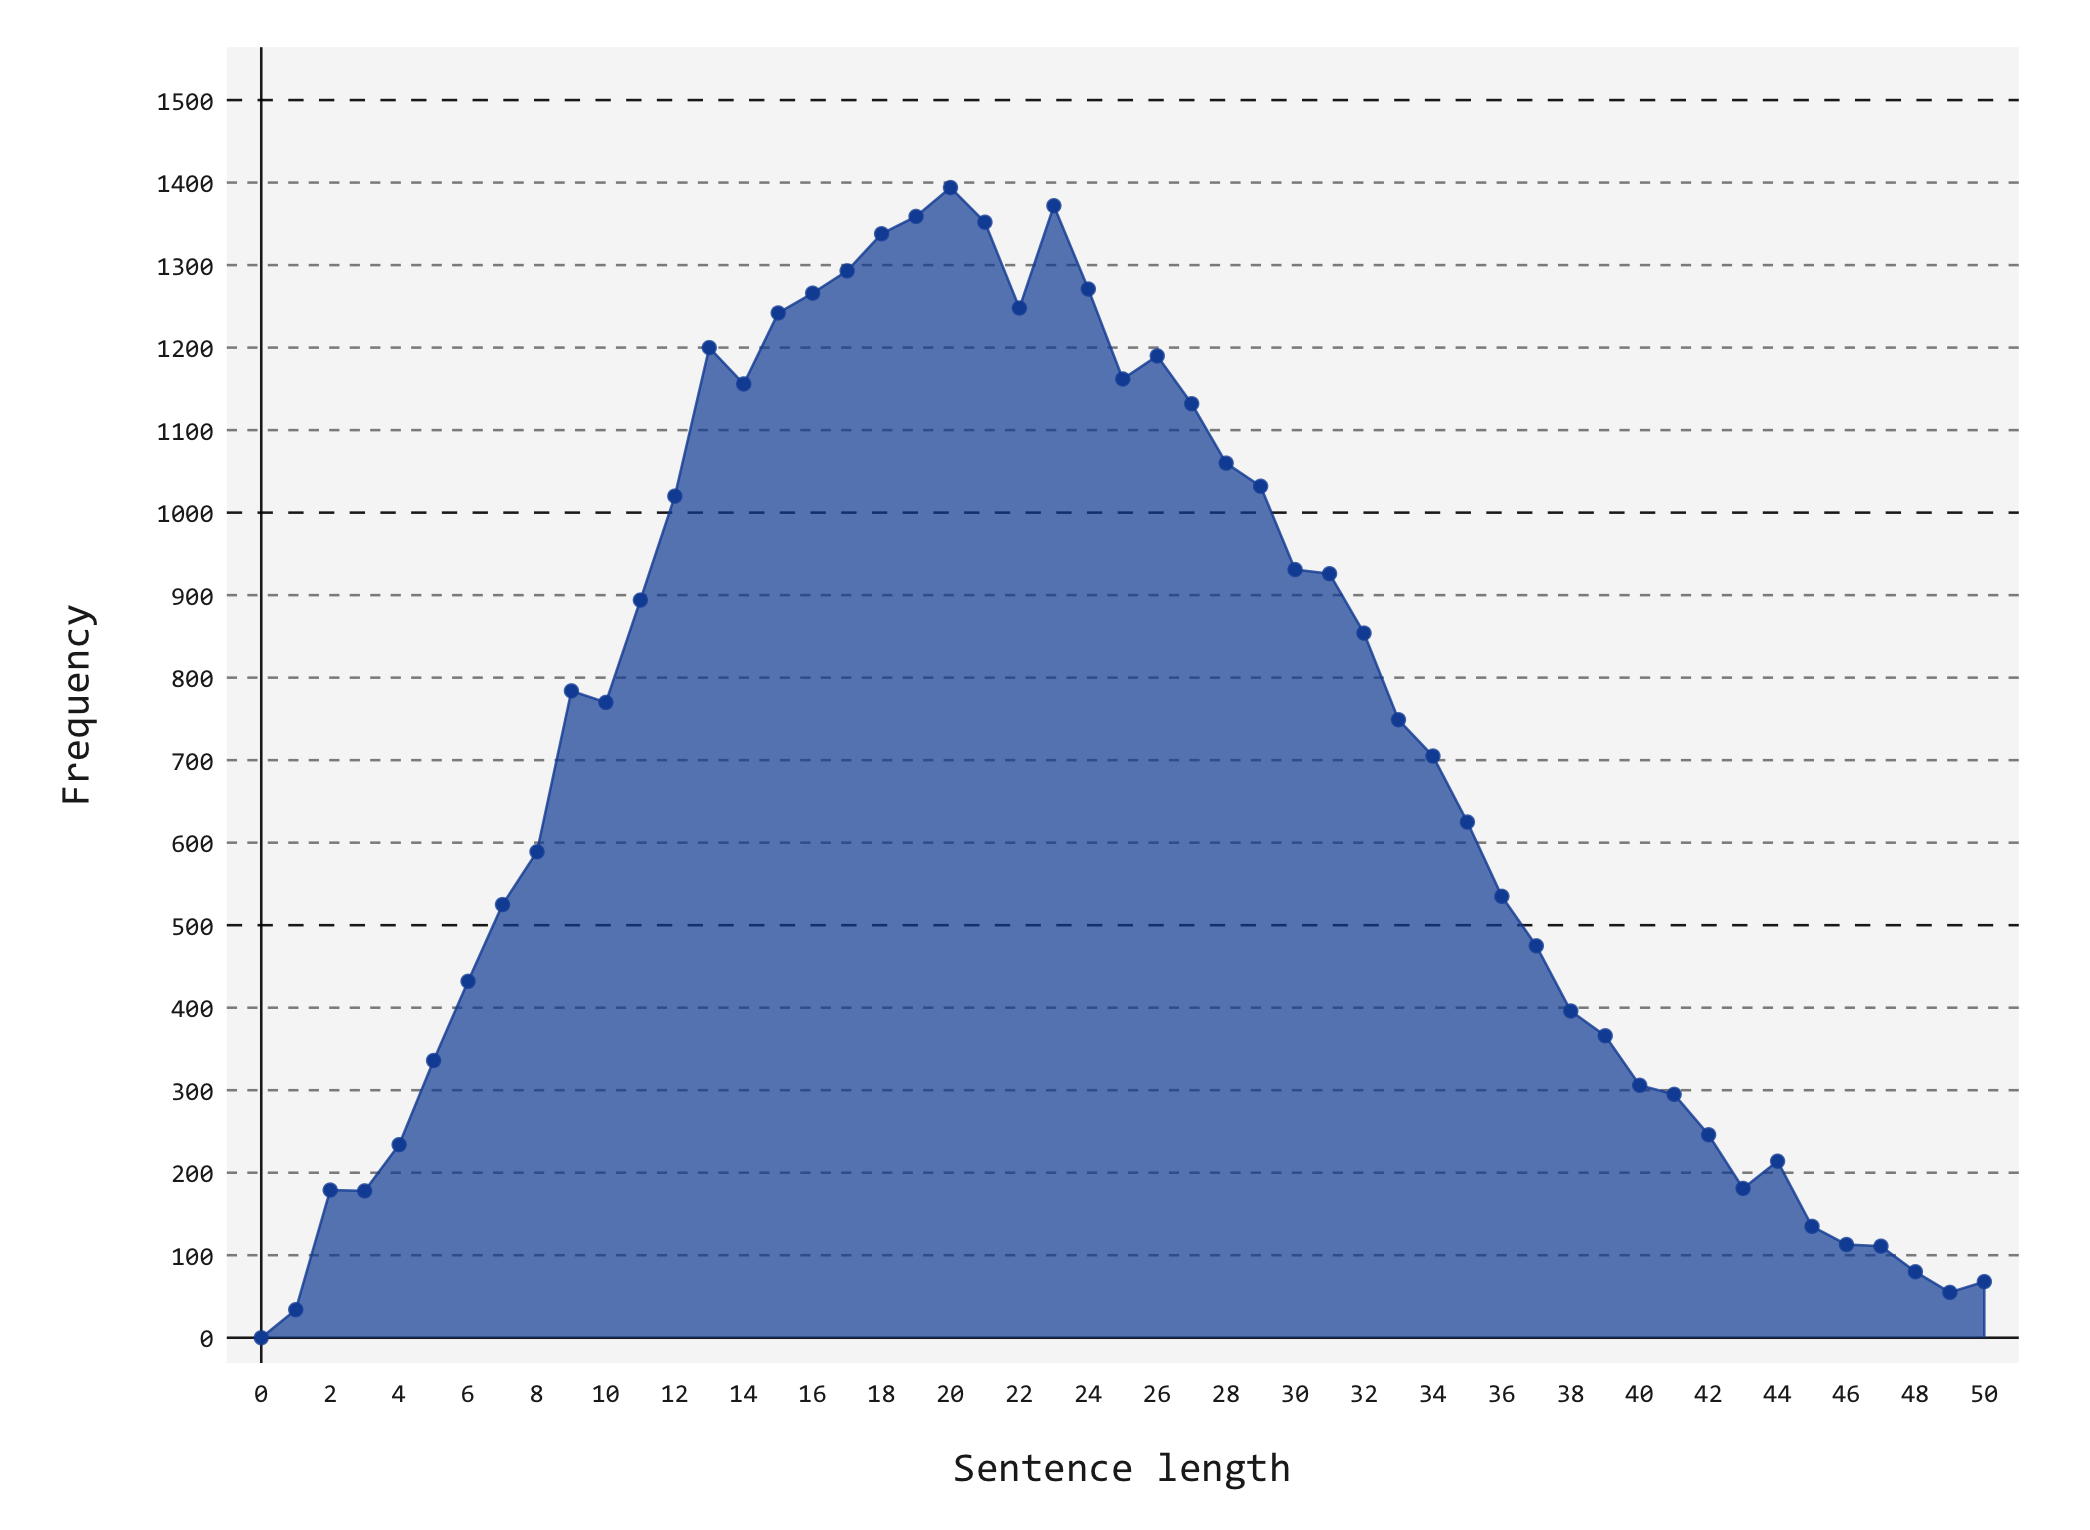
\includegraphics[width=\textwidth]{s_length_training}
    \end{minipage}\hfill
    \caption{Distribution of sentence lengths and their frequency in the training data.}
    \label{fig:sentence_length_1}
\end{figure}

\begin{figure}[h]
    \centering
    \begin{minipage}{0.8\textwidth}
        \centering
        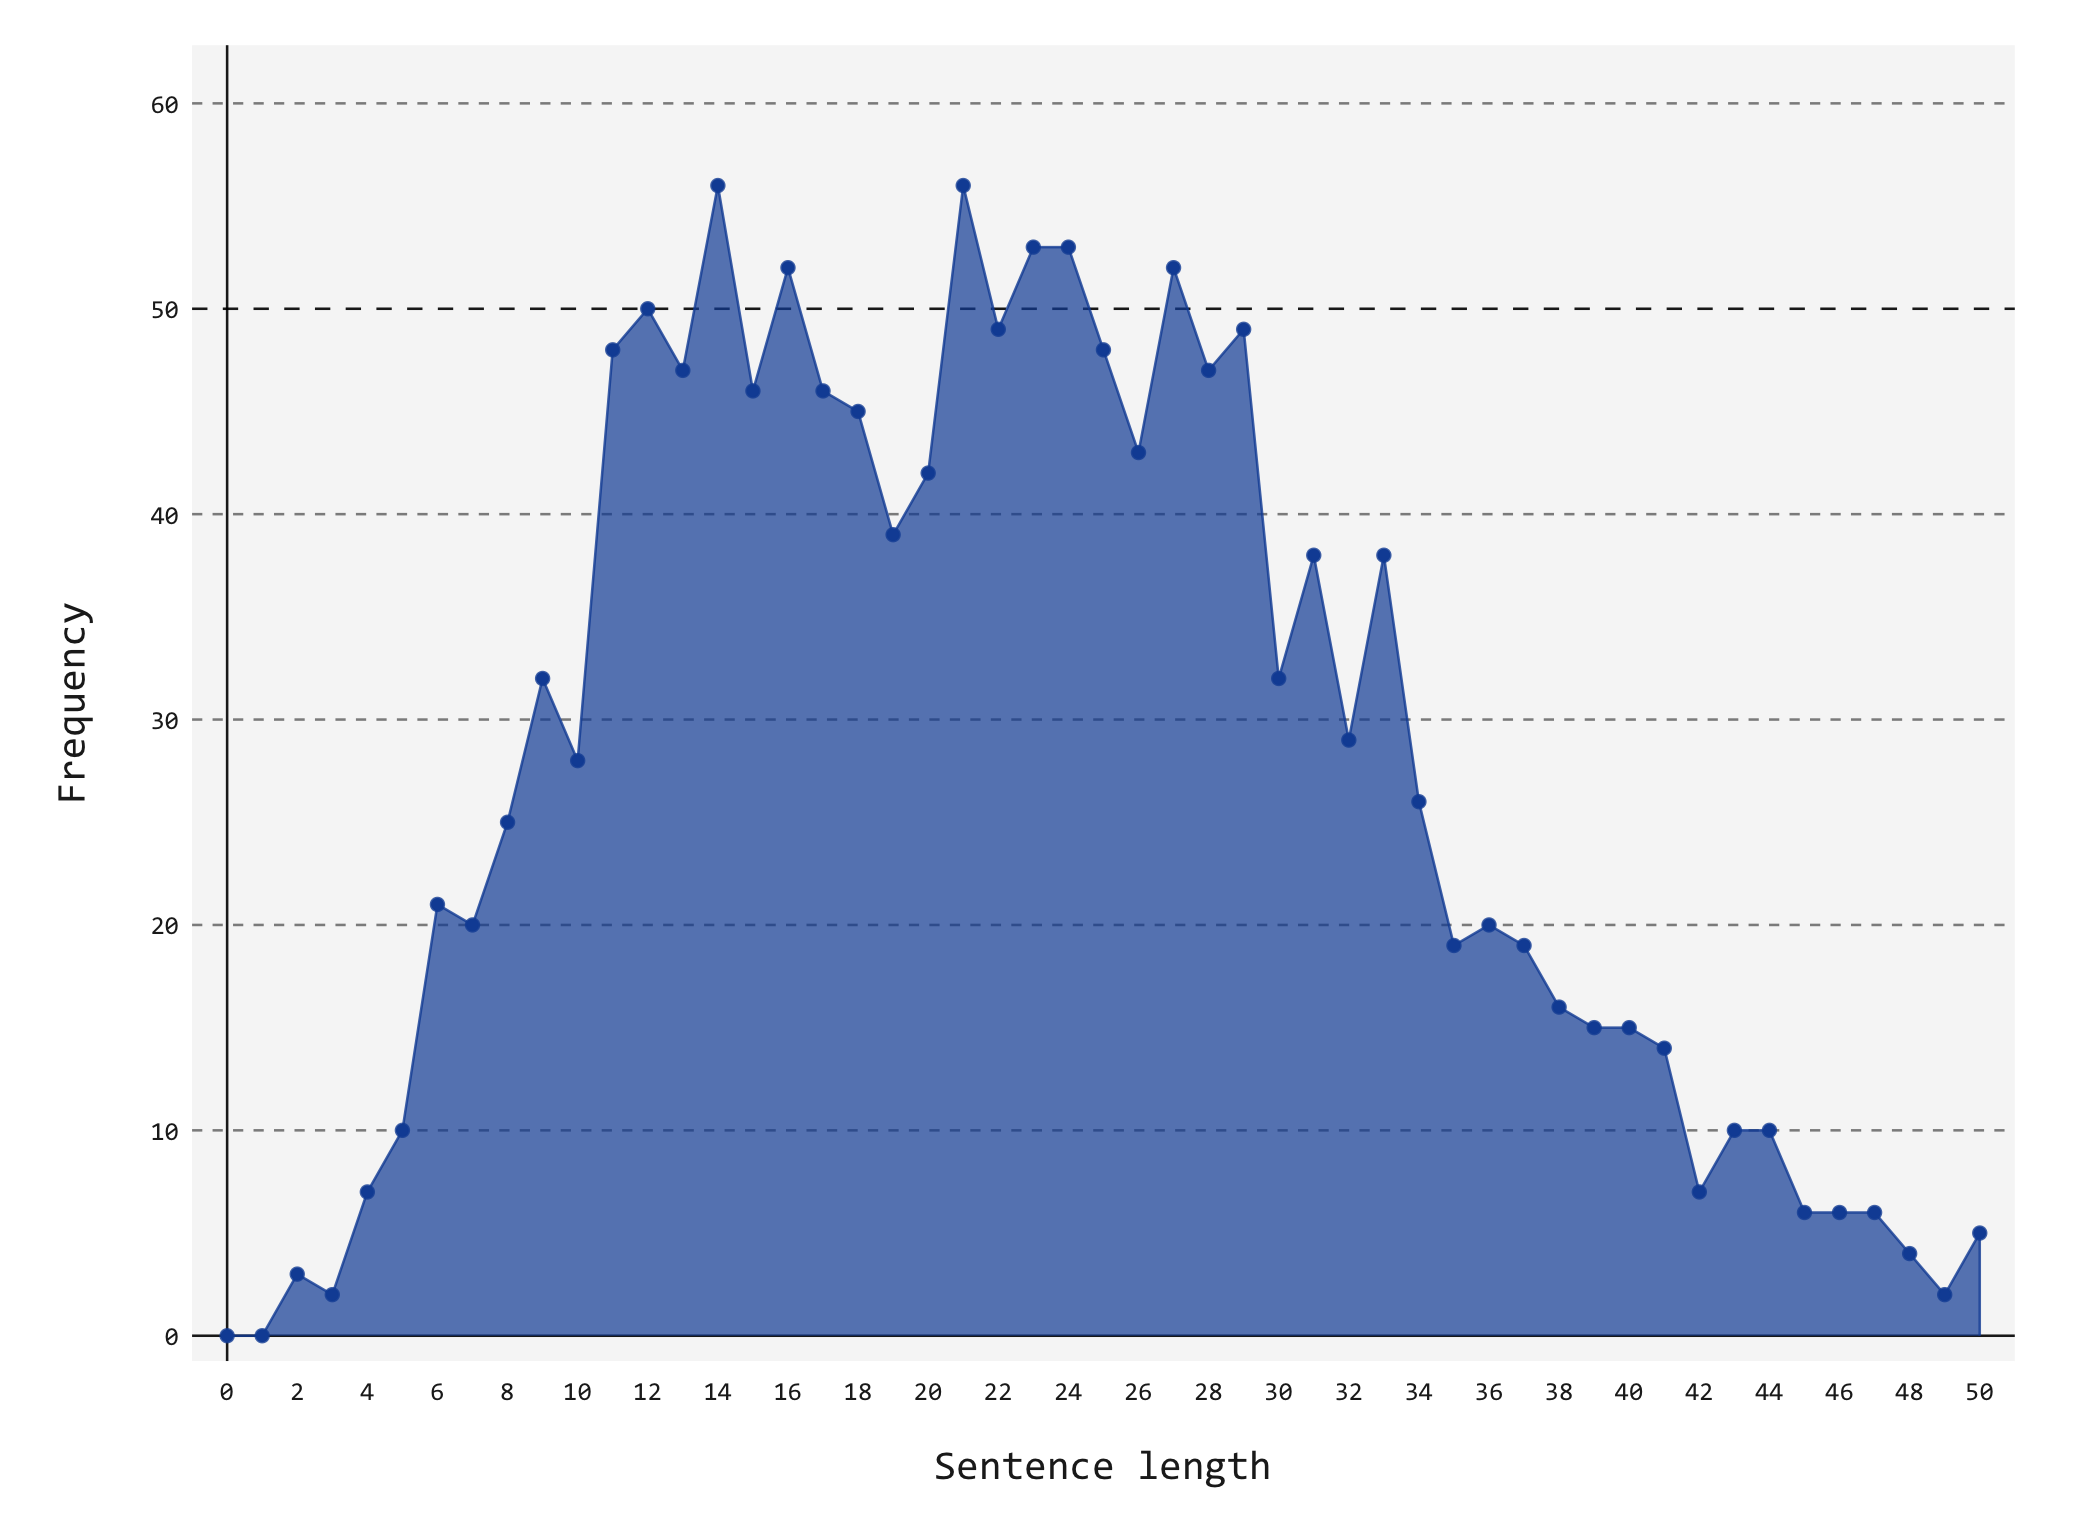
\includegraphics[width=\textwidth]{s_length_testing}
    \end{minipage}
    \caption{Distribution of sentence lengths and their frequency in the test data.}
    \label{fig:sentence_length_2}
\end{figure}

\begin{table}
    \centering
    \begin{tabular}{@{}cccccccccc@{}}
        \toprule
        \multicolumn{1}{c}{ }
        & \multicolumn{1}{c}{ }
        & \multicolumn{4}{c}{\textbf{DM}}
        & \multicolumn{4}{c}{\textbf{PSD}} \\
        \cmidrule(lr){3-6}
        \cmidrule(lr){7-10}
        &
        LF.av &
        LF & LP & LR & FF &
        LF & LP & LR & FF \\
        \midrule
        Peking & 85.33 & 89.09 & 90.93 & 87.32 & 63.08 & 75.66 & 78.60 & 72.93 & 49.95 \\
        Lisbon & 85.15 & 88.21 & 89.84 & 86.64 & 00.15 & 76.36 & 78.62 & 74.23 & 00.03 \\
        \midrule
        Lisbon* & 86.23 & 89.44 & 90.52 & 88.39 & 00.20 & 77.58 & 79.88 & 75.41 & 00.06 \\
        Turku* & 83.47 & 86.17 & 87.80 & 84.60 & 54.67 & 73.63 & 76.10 & 71.32 & 53.20 \\
        \bottomrule
        
        \\
        \toprule
        \multicolumn{1}{c}{ }
        & \multicolumn{1}{c}{ }
        & \multicolumn{4}{c}{\textbf{DM}}
        & \multicolumn{4}{c}{\textbf{PSD}} \\
        \cmidrule(lr){3-6}
        \cmidrule(lr){7-10}
        &
        LF.av &
        LF & LP & LR & FF &
        LF & LP & LR & FF \\
        \midrule
        Lisbon & 81.15 & 81.75 & 84.81 & 78.90 & 00.27 & 74.82 & 78.68 & 71.31 & 02.09 \\
        Peking & 80.78 & 81.84 & 84.29 & 79.53 & 47.49 & 73.28 & 77.36 & 69.61 & 34.28 \\
        \midrule
        Lisbon* & 82.53 & 83.77 & 85.79 & 81.84 & 00.35 & 76.18 & 80.12 & 72.61 & 02.25 \\
        Turku* & 78.85 & 79.01 & 81.54 & 76.63 & 39.15 & 71.59 & 74.92 & 68.55 & 38.75 \\
        \bottomrule
    \end{tabular}
    \caption{SemEval-2015 results from the closed track (unmarked) and open track (marked *) of the in-domain (top) and out-of-domain (bottom) data for the three parsers included our the analysis.}
    \label{fig:data:recap}
\end{table}

In Chapter \ref{chap:semantic} we reviewed the technical aspects of the three parsing systems we will examine here. The Peking system: an ensemble of transition-based and graph-based models, the Turku system: a combination of several classifiers for classifying specific aspects of the semantic dependency graphs, and the Lisbon system: a graph-based feature-rich linear model that parametrize globally over first and second order dependencies.

In Table \ref{fig:data:recap} we see data on the accuracy of the three parsing systems. A somewhat obvious aspect of these results is that the parsing systems perform better on the in-domain versus the out-of-domain data sets. This is to be expected, as data-driven parsing will yield better results on data that is within the domain of the data used for training. In terms of the specific types of errors we examine: length, graph and linguistic factors, there is an overall drop from in-domain to out-of-domain data, but no statistically significant changes in the relative error rate between the different factors. So we expect the results of our analysis to be the same if we had chosen to examine the out-of-domain data sets, with the significant difference being the overall lower scores.

We have therefore chosen to solely focus on the results for the in-domain data. Our research has set out to explore the specific errors that different parsing systems make. We are therefore less interested in the errors that are related to factors that might be attributed to corpora, such as type of vocabulary, size of vocabulary, differences in sentence structure, and so forth. Such analysis would demand a different type of study where the corpora would also be subject to a comparative analysis.

In SemEval-2015, the parsing could be run in an open and closed track: see Chapter \ref{chap:semantic} for details on these tracks and the approaches used by the parsing systems participating in the open tracks. Lisbon is the only team that participated in both tracks, Peking participated only in the closed track, and Turku only in the open track.\footnote{Turku also participated in the gold track, as the only team. We exclude the gold track from our analysis as it does not provide any significant insights to the comparative nature of our analysis.} For our analysis we have chosen to use data from the open track for Turku, since there is no data for Turku in the closed track, and the closed track for Lisbon and Peking. It is therefore important to note that the comparisons in our analysis must bear in mind that the Turku parsing system has the added benefit of using additional resources such as a syntactic parser: see \citeA{Kanerva:Turku:15} for specific details on the additional resources used by Turku.

Examining Table \ref{fig:data:recap}, we see that the Peking parser performs slightly better than Lisbon on average in the closed track. The Lisbon parser has a higher overall accuracy in the open track, which attests to the fact that using a syntactic parser as additional features for the parsing can increase the overall accuracy of semantic dependency parsing. Even though the Turku parser participated in the open track, its overall accuracy is lower than that of Peking and Lisbon in the closed track. Another observation is that the Peking parsing system has a higher accuracy on the DM target representation, but lower than Lisbon on the PSD target representation. On the out-of-domain data we see that the Lisbon parsing system has the overall highest score. The differences in the overall scores between the Peking and Lisbon parsing systems are marginal. It is therefore interesting to see what the specific differences are when examining the different factors in their own right.

It is worth noting that all three parsing systems have a substantially lower accuracy on the PSD target representation. One of the reasons for this lower overall accuracy on the PSD target representation can be attributed to the higher number of dependency types relative to DM.

\subsection{Measuring parsing accuracy}

The measures used for determining the scores of the submission are \textit{precision}, \textit{recall}, and \textit{f-score}. When calculating these, we use the measures \textit{true positives}: instances that have been correctly predicted, \textit{false positives}: instances that have been falsely identified, and \textit{false negatives}: instances that should have been predicted, but have not been predicted.

Precision, also known as positive predictive value, is a measure for the \textit{reliability} of a system's predictions. These are the dependencies that have been correctly assigned during the parsing. We calculate this as follows:

\begin{equation*}
    \text{Precision} = \frac{\text{true positives}}{\text{true positives + false positives}}
\end{equation*}

\vspace{1ex}

Recall, also known as sensitivity, is the measure for how \textit{robust} a system is. These are the fraction of relevant dependencies that have been assigned during parsing. This measure is calculated as follows:

\begin{equation*}
    \text{Recall} = \frac{\text{true positives}}{\text{true positives + false
            negatives}}
\end{equation*}

\vspace{1ex}

F-score is the so-called \textit{harmonic mean} of the precision and recall, and is calculated as follows:

\begin{equation*}
    \text{F-score} = 2*\frac{\text{precision * recall}}{\text{precision + recall}}
\end{equation*}

\vspace{1ex}

We will now start our error analysis by first examining errors when related to length factors.
    
%%%%%%%%%%%%%%%%%%%%%%%%%%%%%%%%%%%%%%%%%%%%%%%%%%%%%%%%%%%%%%%%%%%%%%%%%%%%%%%%%%%%%%%%%%%%%%%%%%%%%%%%%%%%%%%%%%%
% START
\section{Length factors}

\begin{figure}[h]
    \centering
    \begin{minipage}{0.8\textwidth}
        \centering
        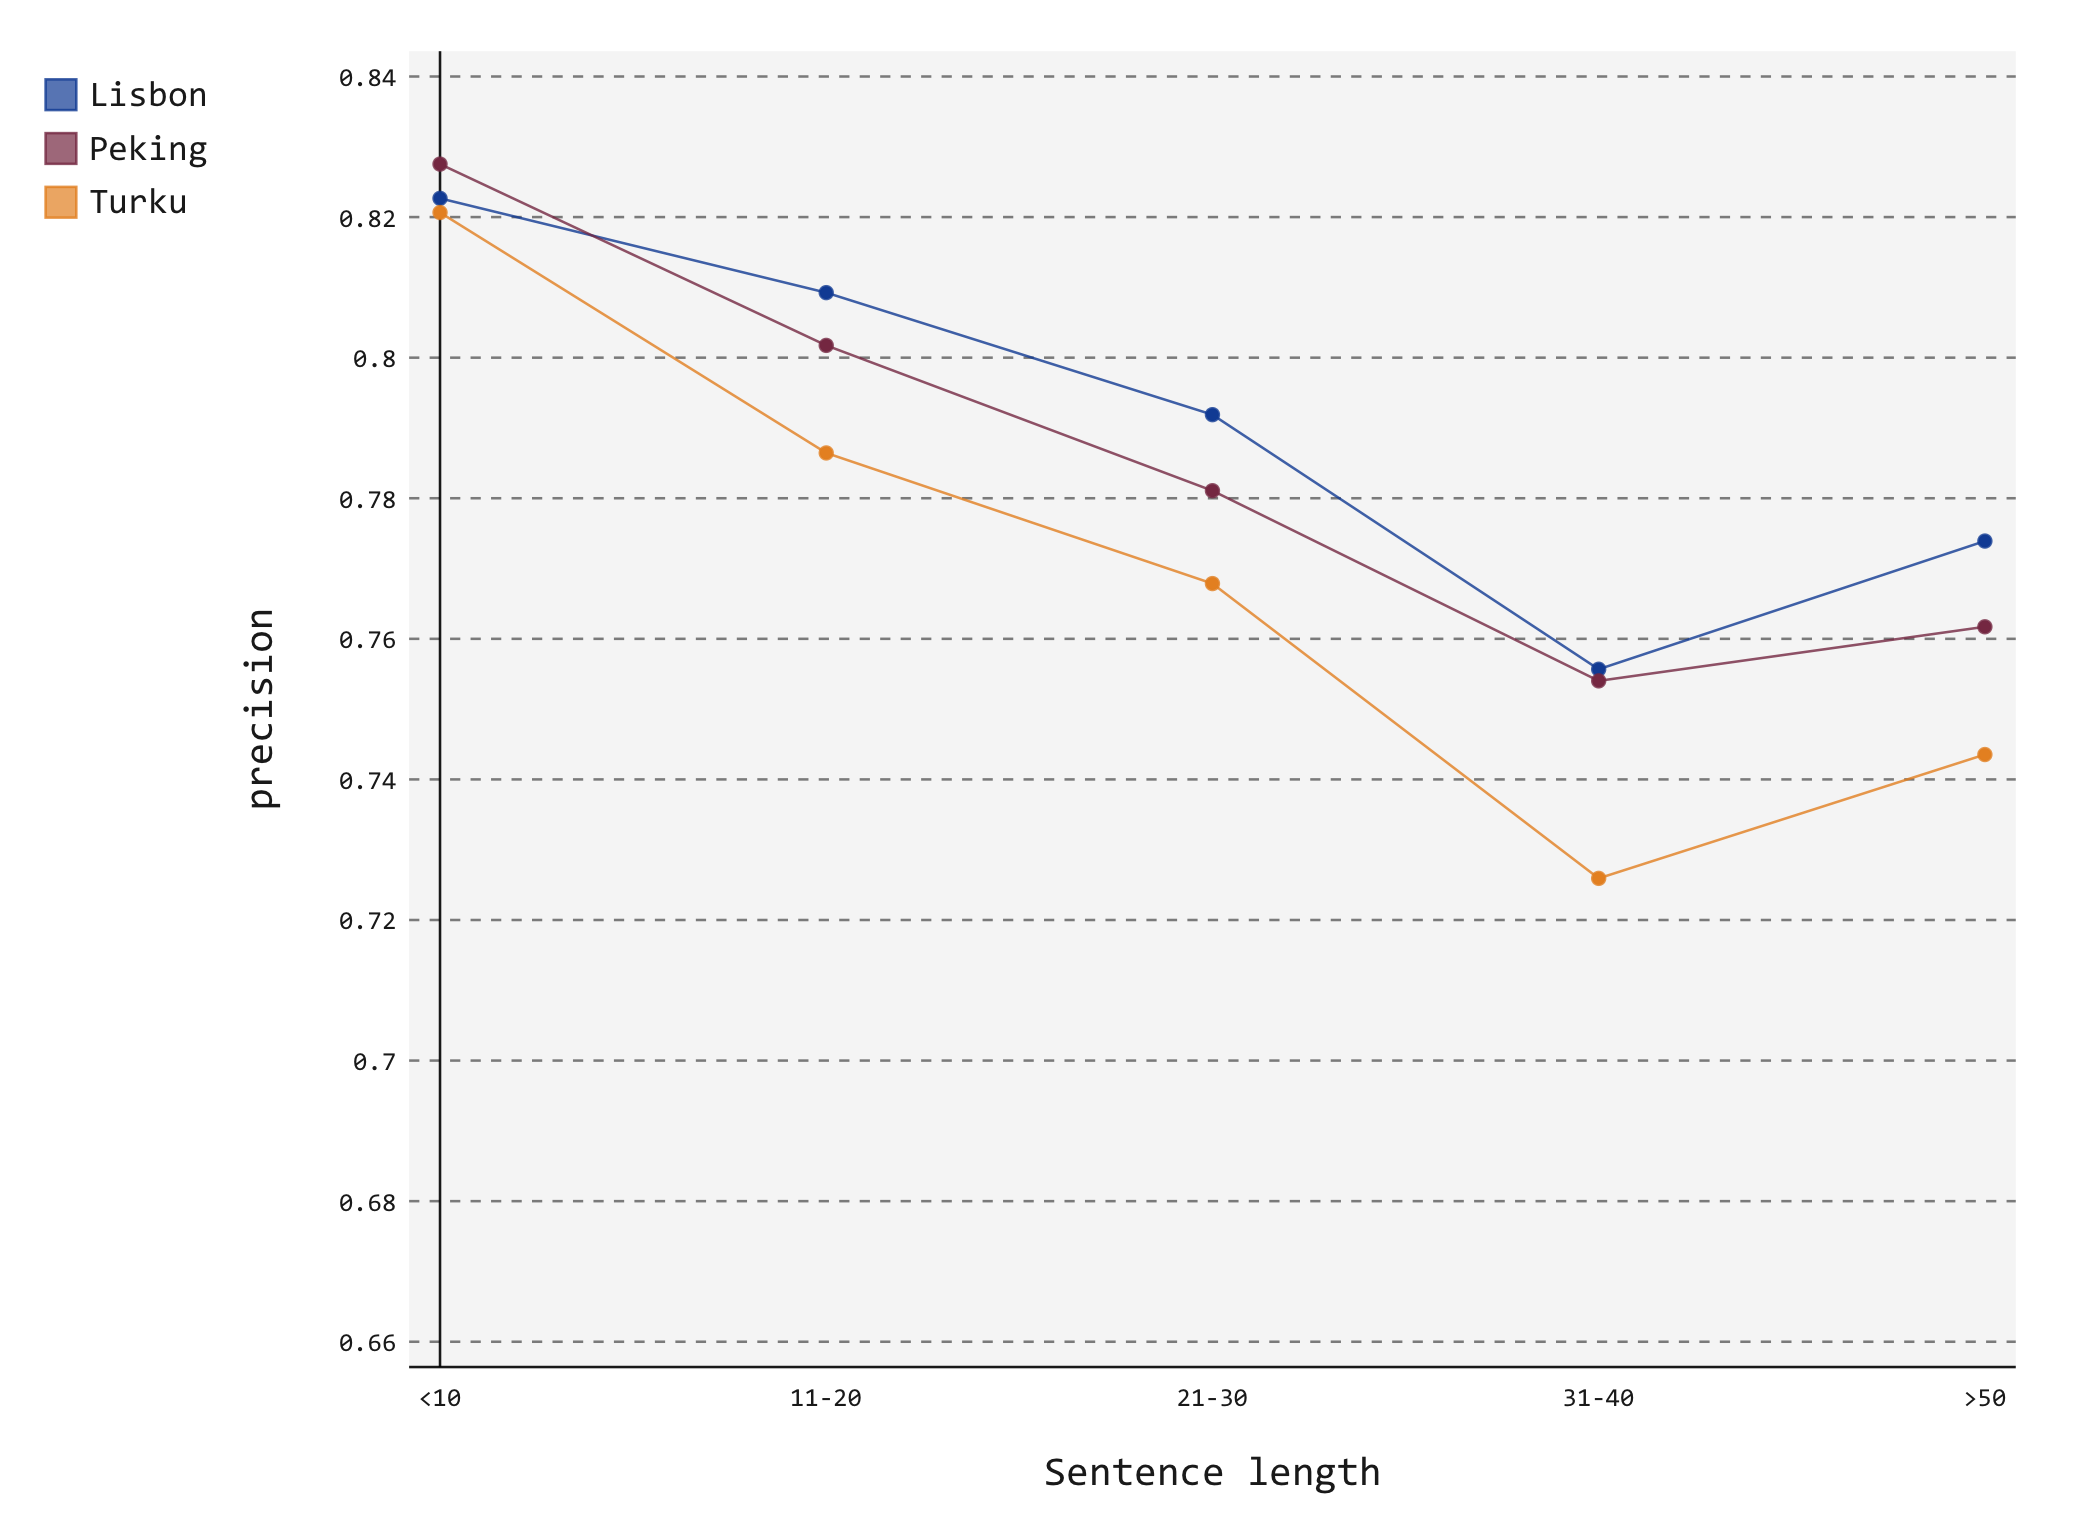
\includegraphics[width=\textwidth]{sentence_length_precision_PSD}
    \end{minipage}
    \caption{Accuracy relative to sentence length in bins of size 10. Precision for the PSD target representation.}
    \label{fig:s_length_PSD_1}
\end{figure}

\begin{figure}[h]
    \centering
    \begin{minipage}{0.8\textwidth}
        \centering
        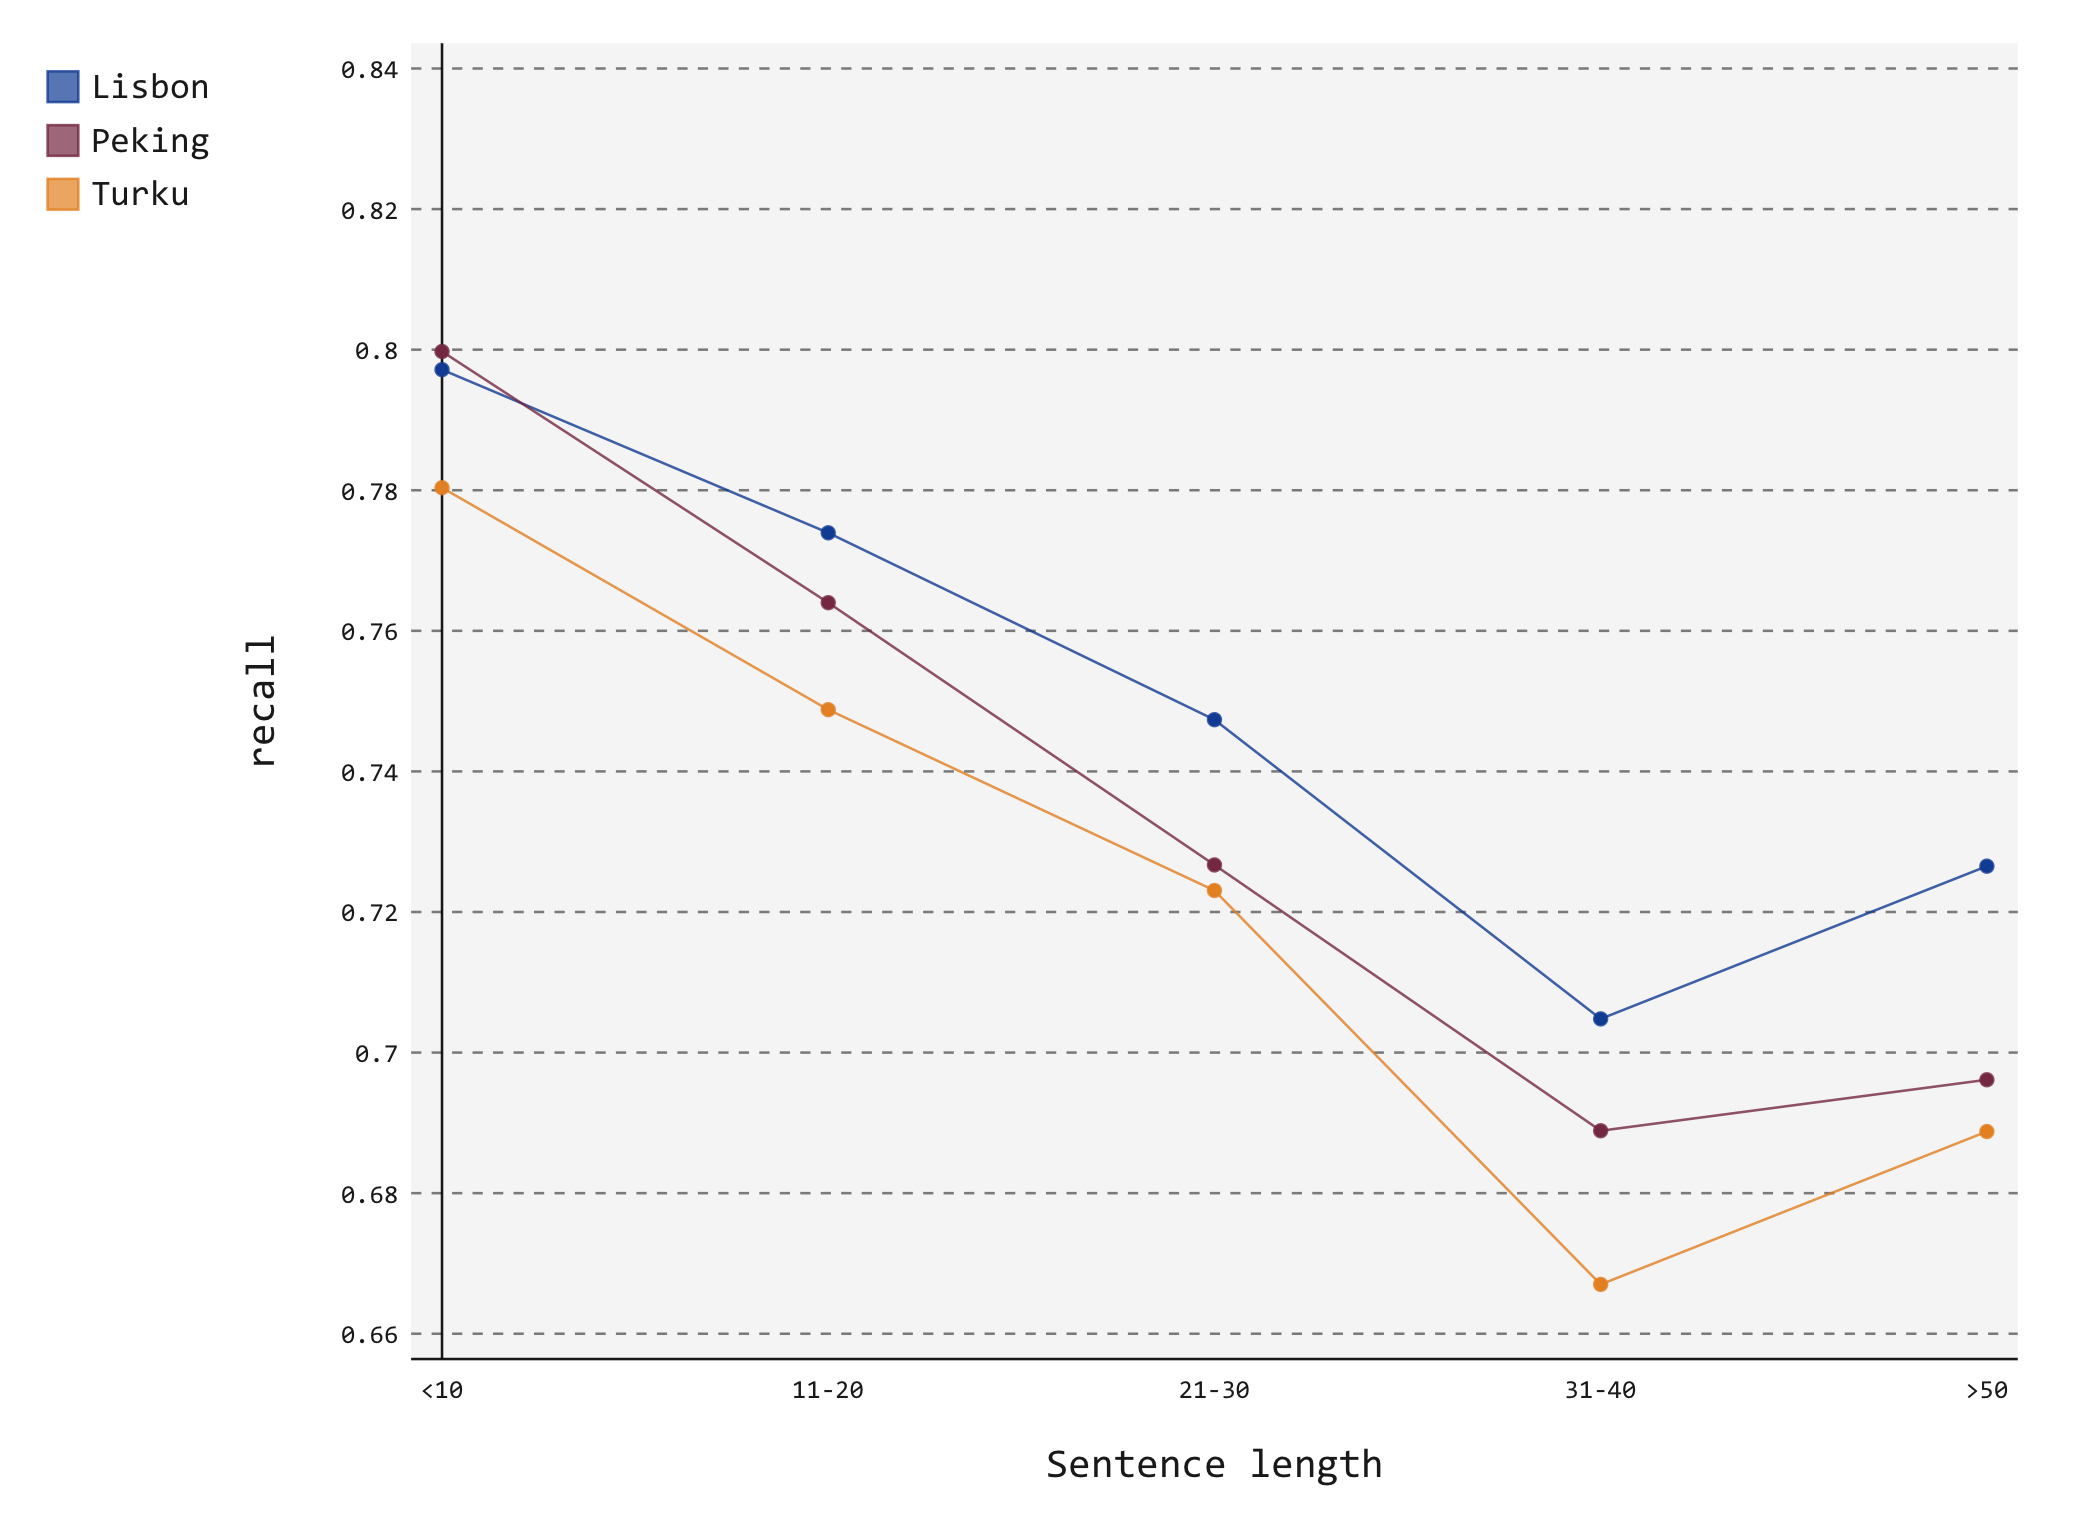
\includegraphics[width=\textwidth]{sentence_length_recall_PSD}
    \end{minipage}\hfill
    \caption{Accuracy relative to sentence length in bins of size 10. Recall for the PSD target representation.}
    \label{fig:s_length_PSD_2}
\end{figure}

As \citeA{McD:Niv:07} point out, it is well known that syntactic parsing systems produce results with lower accuracy for longer sentences. We observe the same phenomena in the results of our three parsing systems: parsing accuracy has an inverse correlation with sentence length. As \citeA{McD:Niv:11} observe, this is primarily due to more complex constructions in longer sentences, such as prepositions, conjunctions, and multi-class sentences.

Another type of length factor is the length of the dependencies themselves. We observe a decrease in parsing accuracy as the length of dependencies increase. We define the length of a dependency from word $w_i$ to $w_j$ as $|j - i|$. In our analysis a length of $0$ is used for the top node. For the English language, and from examining the data sets used in SemEval-2015, we can generally state that short dependencies are modifiers of nouns, such as determiners, adjectives or pronouns. Longer dependencies are in most cases words that modify the main verb or root of the sentence.

\subsection{Sentence length}

In this section we will examine sentence length as a factor of parsing. First we point out the distribution of sentence lengths in the training and test data in Figure \ref{fig:sentence_length}. The distribution approximates the \textit{Bell curve}, and the average sentence length is 22.51 lexical units for the training, and 22.66 for the test data. However, the test data has a distribution where the approximation towards the Bell curve is more crude due to its relatively smaller size.

In Figures \ref{fig:s_length_DM} and \ref{fig:s_length_PSD} we see the precision and recall for the three parsing systems for both the DM and PSD target representations. The graphs in these Figures show precision and recall for sentences in bins of 10. If we look at the DM target representation, we see that the results of Lisbon and Peking are quite similar, where there is a correlation of precision and recall in relation to sentence length. The overall trend is that for longer sentences, the precision and recall of the parsing decreases. This overall trend was also observed by \citeA{McD:Niv:07}, \citeA{McD:Niv:11}, and \citeA{Choi:Tetreaul:Stent:15} when examining syntactic parsers.

However, in comparison to the results from the syntactic dependency parsers examined in the mentioned studies, in our analysis we see a slight upwards bump in precision and recall for the last bin that includes sentences that are longer than 50 lexical units. This can be explained by the fact that there are very few sentences with more than 50 lexical units in the testing data set, and that a slight bump might be attributed to the relatively smaller size of that bin. It is therefore worth noting that changing bin sizes would give us slightly different graphs, but that the overall trend would nonetheless be a slight decrease in accuracy as sentence lengths grow.

Another factor that can impact the bump in the last bin is that for semantic dependency graphs we might actually be dealing with two or more disjoint graphs. For sentences that have more than 50 lexical units, a sentence might produce a semantic dependency graph that would be similar to that of two sentences.

Studying the graphs in Figures \ref{fig:s_length_DM} and \ref{fig:s_length_PSD}, we observe that the Lisbon and Peking systems share quite a similar trajectory for both the DM and PSD target representations, with only subtle differences. The Peking parsing system performs better on the DM target representation, while the Lisbon parsing system performs better on the PSD target representation. However, for sentences smaller than 10 lexical units, the Peking parsing system has a higher precision and recall than Lisbon on the PSD target representation. On the DM target representation the trend is in the opposite side, where the Lisbon parsing system outperforms Peking on sentences that are longer than 50 lexical units. Further study of the technical differences in these two parsing systems might shed more light on this phenomena.

Turku on the other hand has an overall different trajectory in comparison to the other two parsing systems on the DM target representation. The largest deviation from the overall trend is that the Turku system, when parsing on the DM target representation, show a particularly low precision and recall on sentences that have lower than 10 lexical units. This is not present when parsing on the PSD target representation, and should be considered an anomaly that might be attributed to some technical detail of the Turku parsing system.

% In Figures \ref{fig:dm_s_length} and \ref{fig:psd_s_length}, we have graphs for the precision and recall of the three parsing systems for both the DM and SDP target representations. As \citeA{McD:Niv:07}, \citeA{McD:Niv:11}, and \citeA{Choi:Tetreaul:Stent:15} found when examining various syntactic parsers, there is also a correlation between sentence length and the accuracy of semantic dependency parsing systems. The longer the sentence, the lower the precision and recall of the results.

% If we look at Figure \ref{fig:dm_s_length}, we see a sharp increase from sentences consisting of more than 3 to 5 lexical units, and then an overall slight reduction of precision and recall as we get longer sentences. We can also observe that the recall is affected to a higher degree than precision, indicating that at parsing, the produced graphs have more dependencies than the gold standard. 

% The correlation between sentence length and precision/recal is more prevalent for the PSD target representation. If we go back to Figure \label{fig:data} from Chapter \ref{chap:semantic}, we see that the PSD target representation has 91 labels, whereas DM has 59. This accounts for some of the reduction in precision and recall that we observe in the results on these two target representations. Examining Figure \ref{fig:psd_s_length}, we see that there is a steeper reduction in both precision and recall for PSD in comparison to DM. We can possibly conclude that the number of dependency types, i.e. the coarseness vs fineness of the dependencies, has a marked impact on the results of parsing systems. This is something that we return to below. 

% Sentence lengths

\subsection{Dependency length}

\begin{figure}[h]
    \centering
    \begin{minipage}{0.8\textwidth}
        \centering
        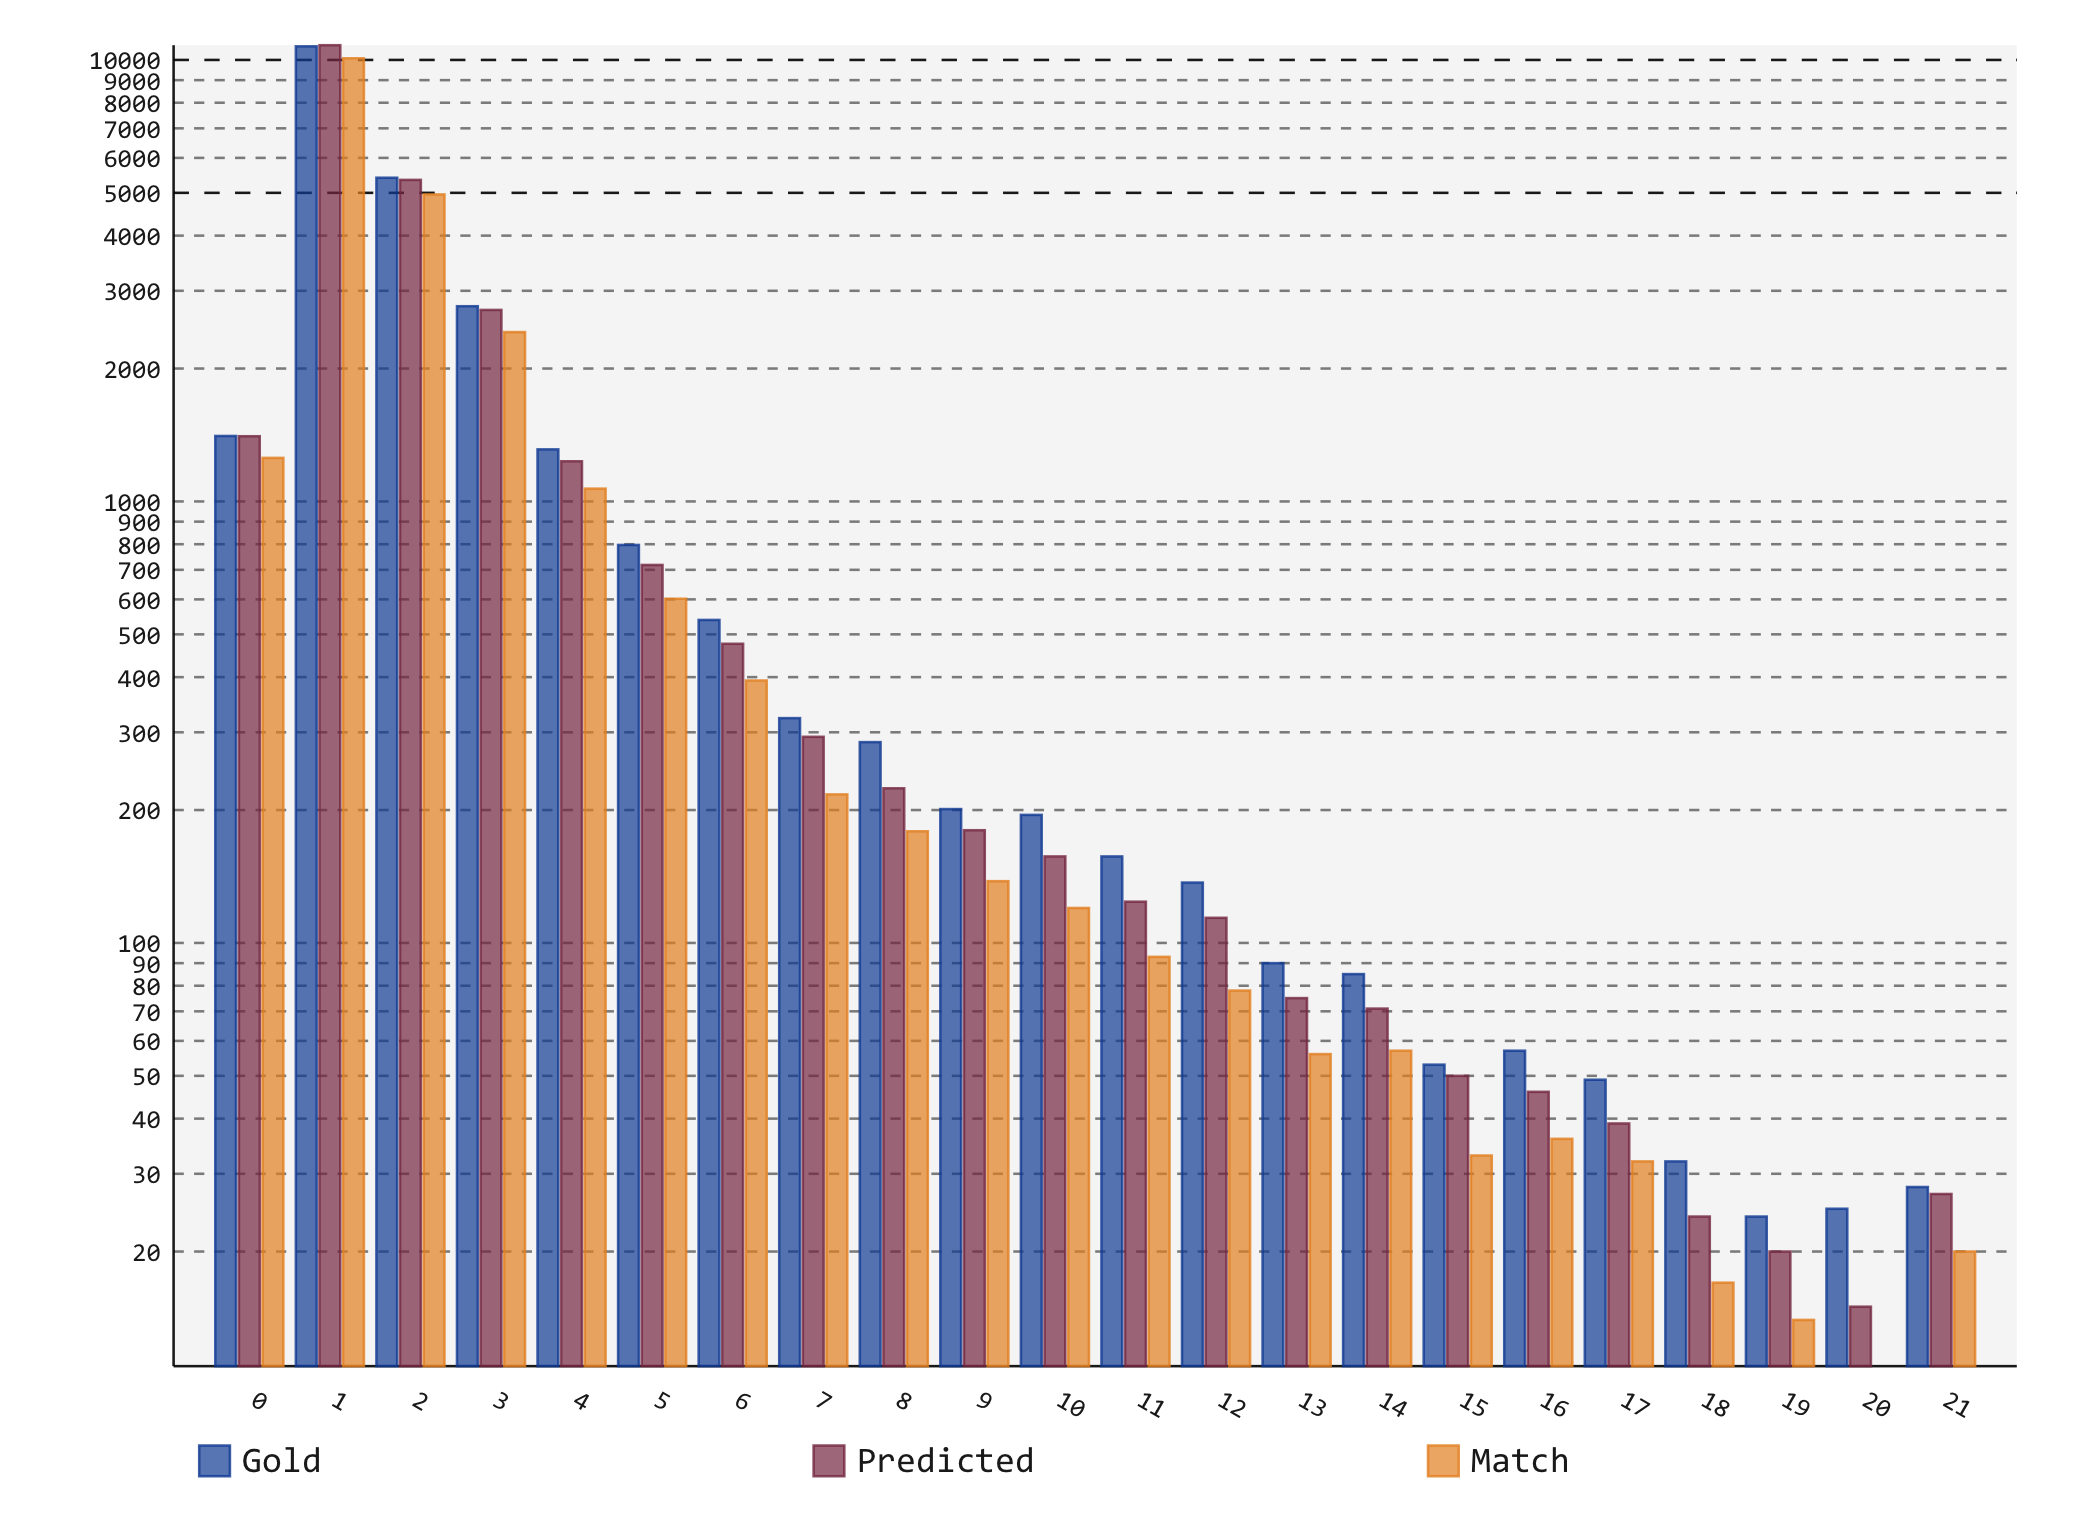
\includegraphics[width=\textwidth]{Lisbon_dep_len_DM}
    \end{minipage}\hfill
    \caption{The number of dependencies for the Lisbon parsing system according to their length (where 0 denotes top nodes) for the DM target representation. The graph shows the number of dependencies in the gold data set, the predicted dependencies, and the matches between predicted and gold.}
    \label{fig:Lisbon_dep_len_DM}
\end{figure}

\begin{figure}[h]
    \centering
    \begin{minipage}{0.8\textwidth}
        \centering
        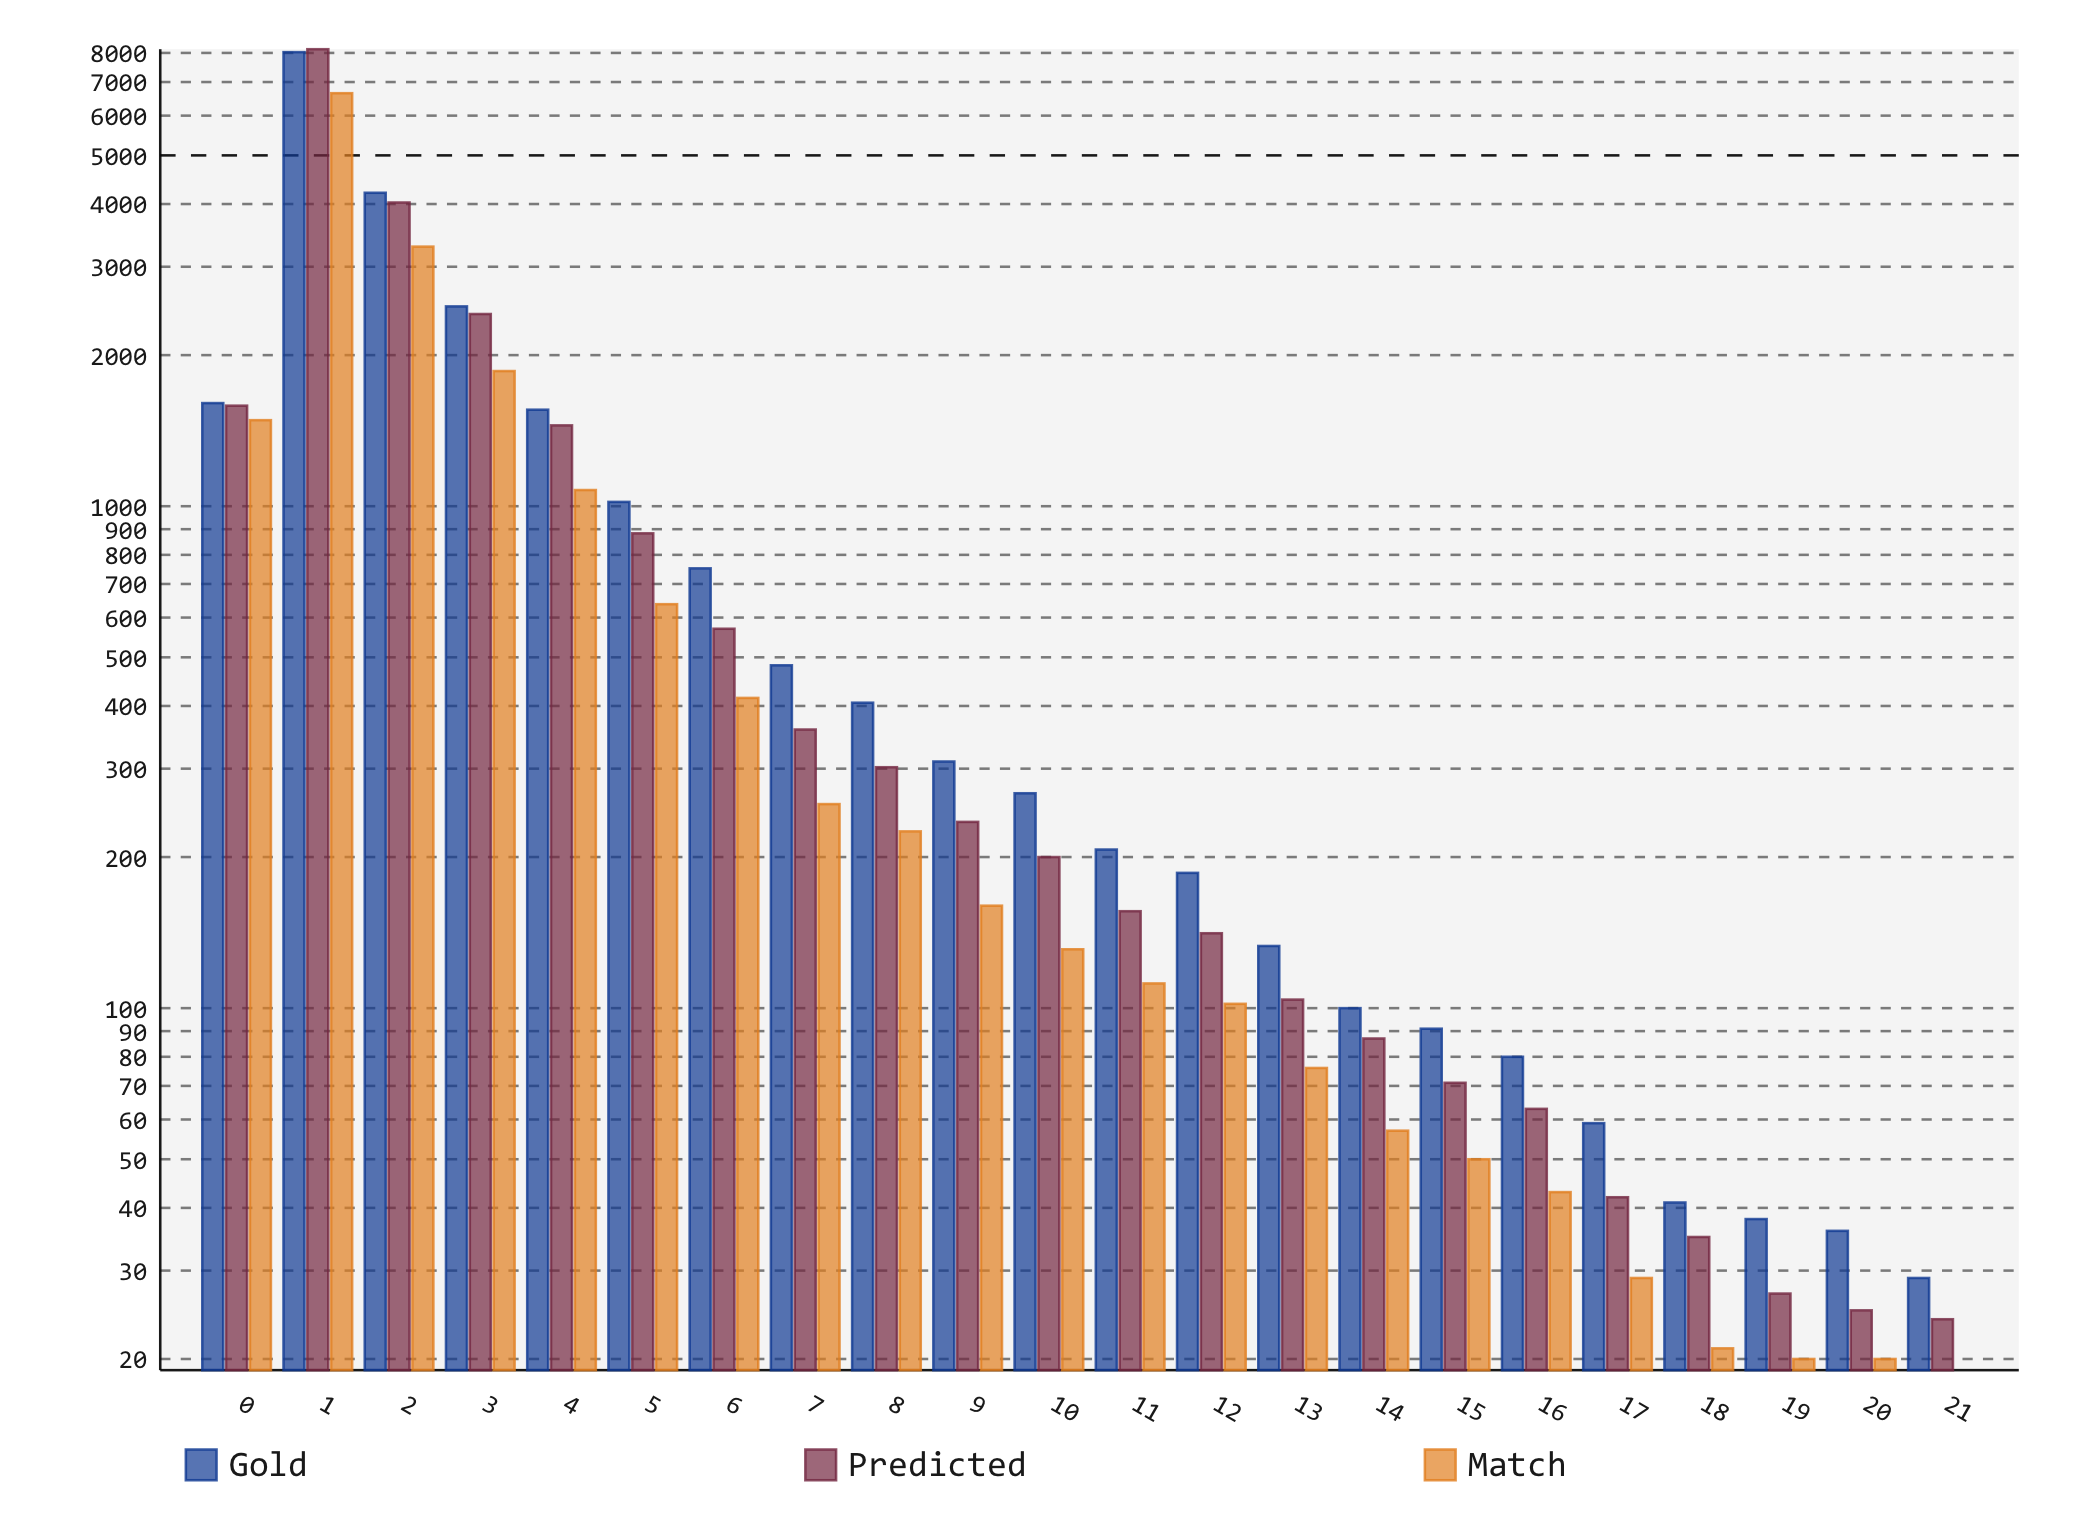
\includegraphics[width=\textwidth]{Lisbon_dep_len_PSD}
    \end{minipage}
    \caption{The number of dependencies for the Lisbon parsing system according to their length (where 0 denotes top nodes) for the PSD target representation. The graph shows the number of dependencies in the gold data set, the predicted dependencies, and the matches between predicted and gold.}
    \label{fig:Lisbon_dep_len_DM}
\end{figure}

\begin{figure}[h]
    \centering
    \begin{minipage}{0.8\textwidth}
        \centering
        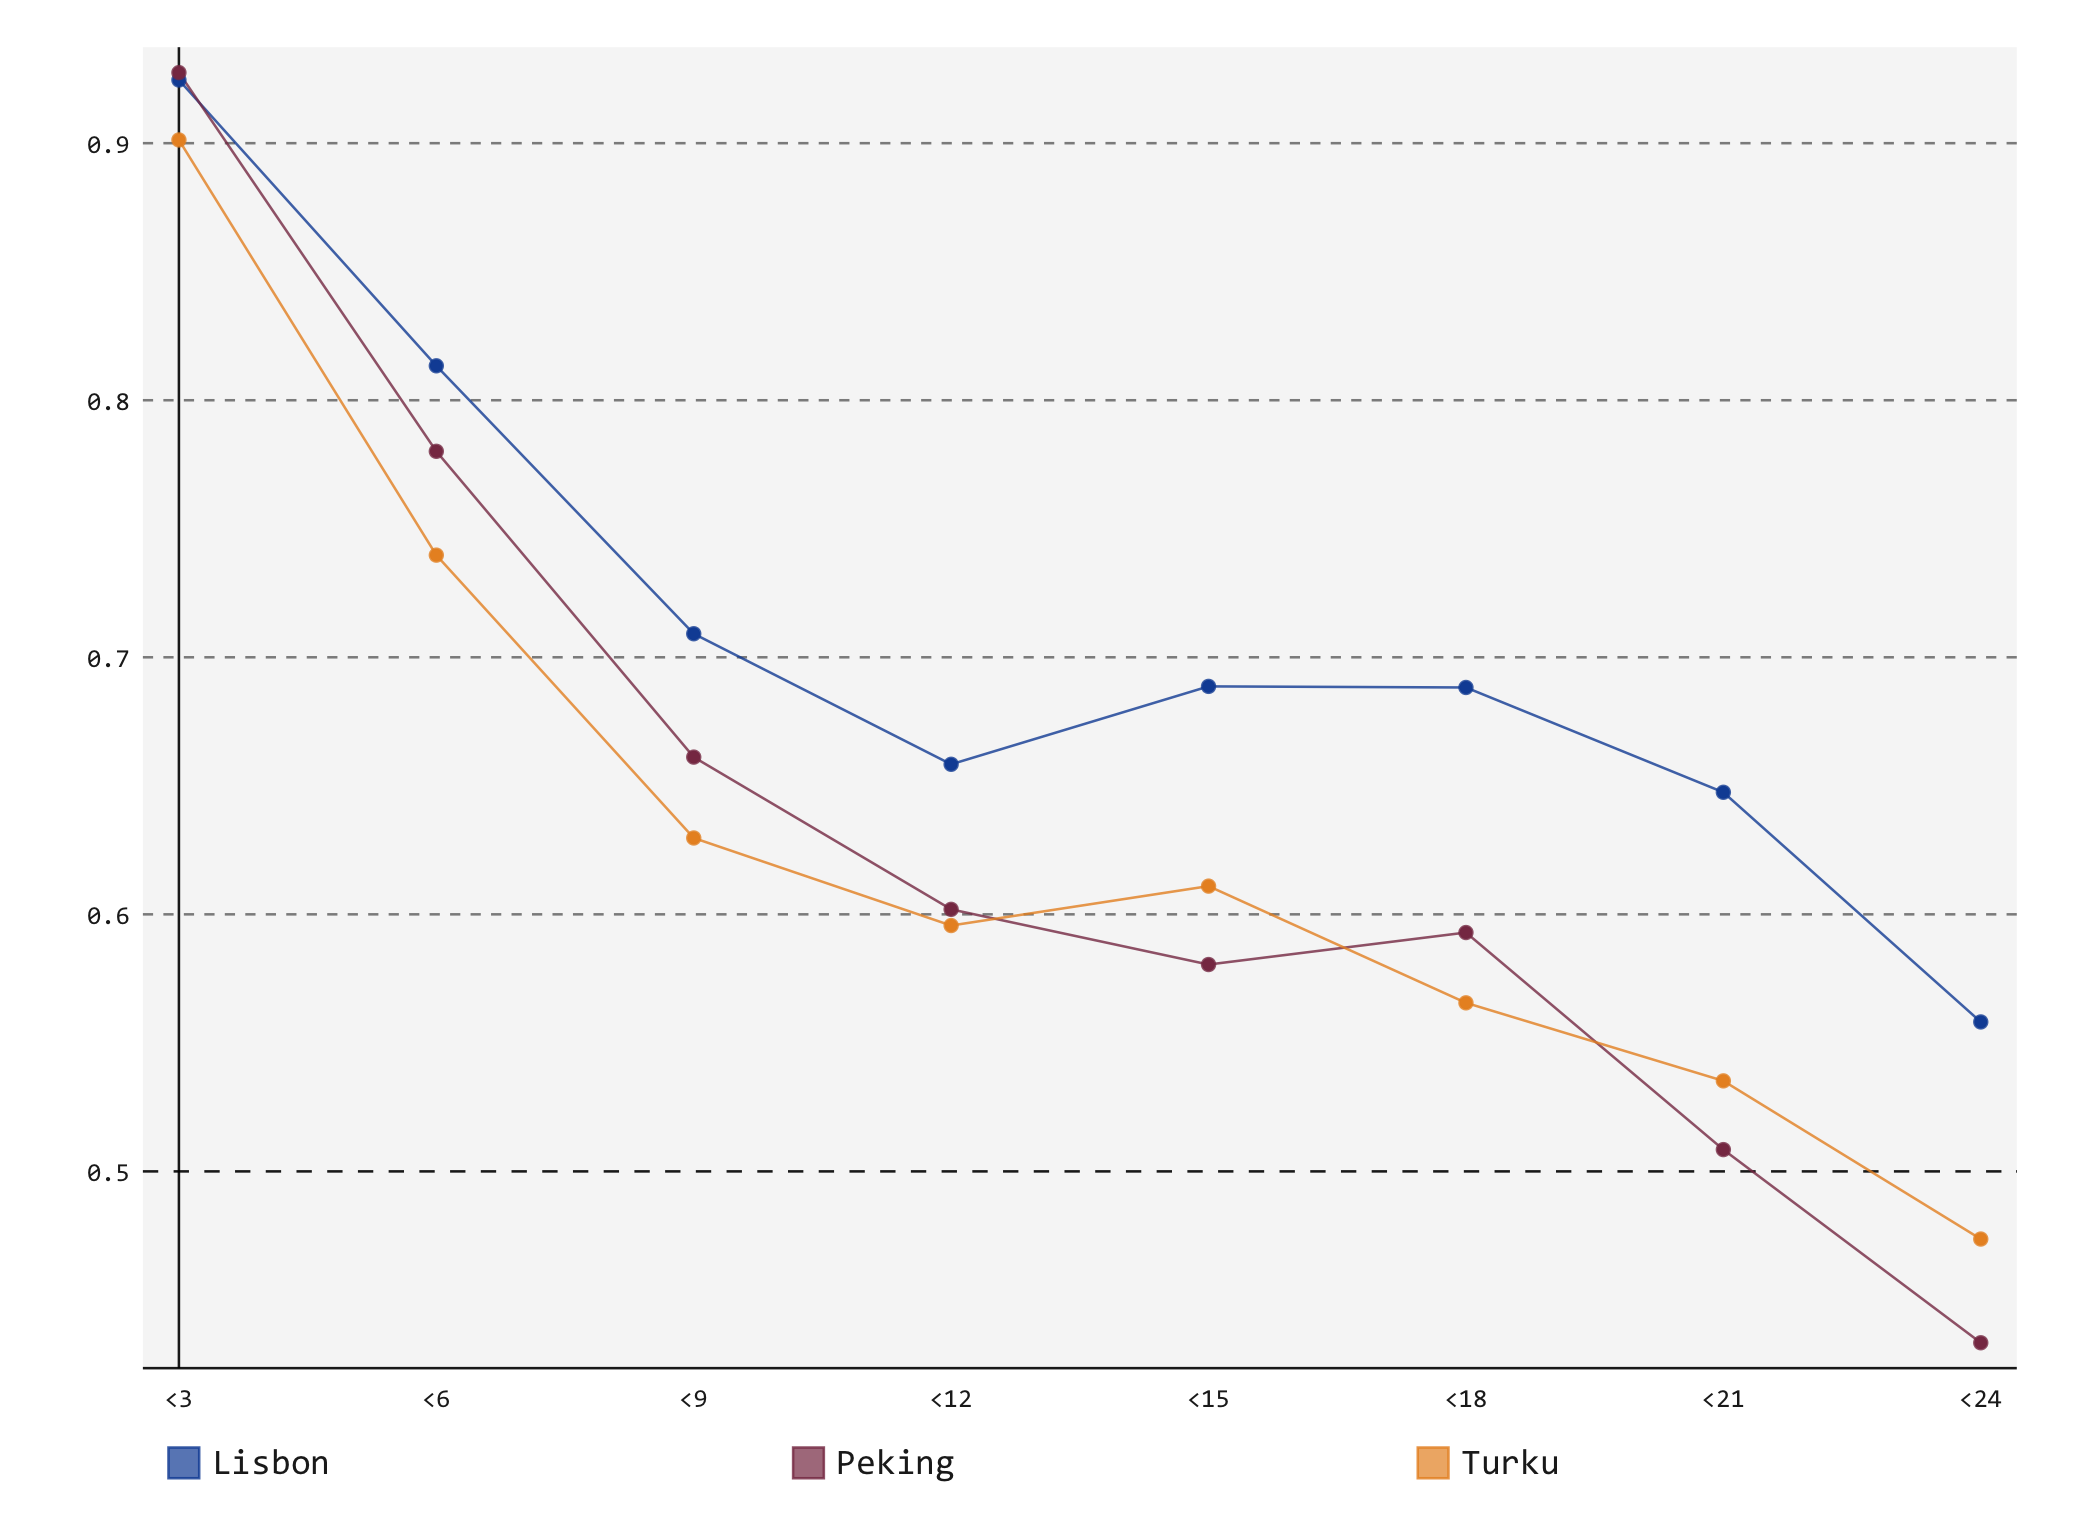
\includegraphics[width=\textwidth]{dep_len_fscore_DM}
    \end{minipage}\hfill
    \caption{F-score for the three parsing systems on the DM target representations for dependency length in bins of 3.}
    \label{fig:dep_len_fscore}
\end{figure}

\begin{figure}[h]
    \centering
    \begin{minipage}{0.8\textwidth}
        \centering
        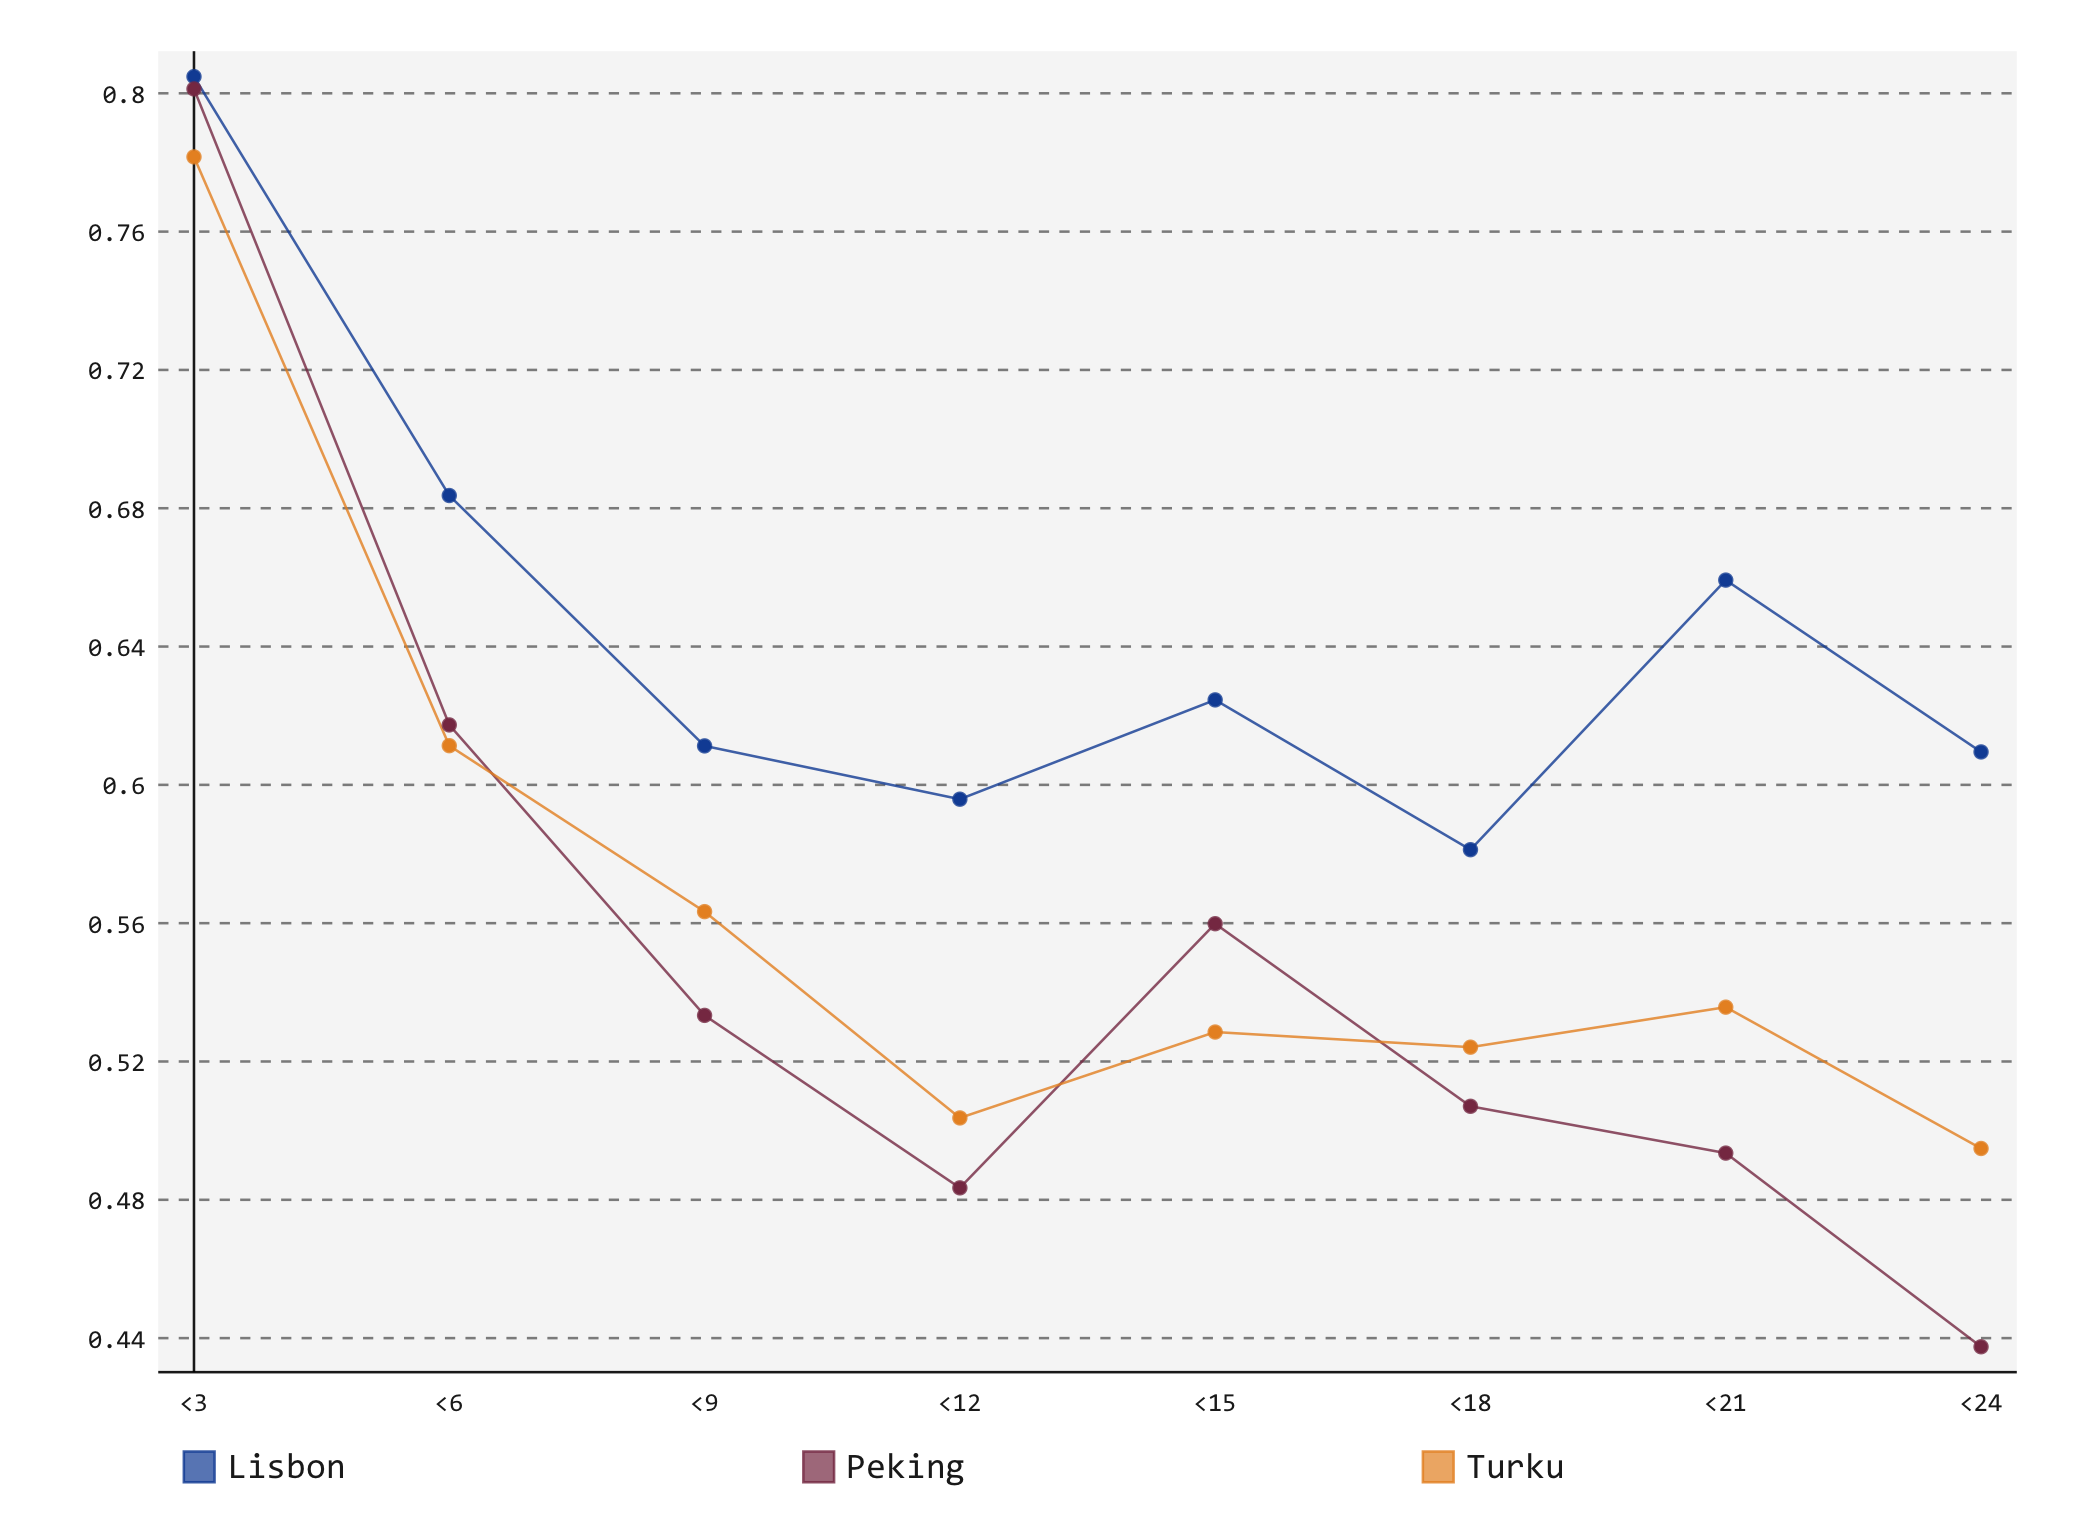
\includegraphics[width=\textwidth]{dep_len_fscore_PSD}
    \end{minipage}
    \caption{F-score for the three parsing systems on the PSD target representations for dependency length in bins of 3.}
    \label{fig:dep_len_fscore}
\end{figure}

Another interesting phenomena is the accuracy of a parsing system relative to the length of dependencies. If we observe the graphs in Figure \ref{fig:Lisbon_dep_len_DM}, we see two graphs representing the number of dependencies of each length for the Lisbon parsing system. The graphs have a distribution over the dependencies in the gold data, the predicted dependencies, and the matches between the gold and predicted data (the correct predictions by the parser).

The most obvious observation on the graphs in Figure \ref{fig:Lisbon_dep_len_DM} is that the Lisbon parsing system consequently makes fewer predictions than what is found in the gold standard data set. The exception occurs when dealing with shorter dependencies, and examining dependencies of length 1 (a dependency between adjacent words), we observe that there are more dependencies in the predictions than gold standard data. As the length of dependencies increase, the number of predictions and matches decrease. These same observations hold for the Peking and Turku parsing systems.

To further elaborate on this point, we introduce the F-score of all parsing systems in relation to dependency length in Table \ref{fig:dep_len_fscore}. Here we have divided dependency length in bins of 3 in order to make the graphs more readable. In regards to f-score in comparison to dependency length we observe that the Lisbon parsing system perform substantially better then the Peking and Turku parsing systems. Peking and Turku have somewhat similar results, with Peking having higher f-score when dependency lengths are between 1 and 12, but actually worse for dependencies above 12 (overall). This might be explained by the fact that Turku participated in the open track, and thus had access to other resources such as a syntactic parser. It might also be due to technical details of the parsing systems.

All three parsing systems demonstrate a decline in f-score as dependency lengths increase on both the DM and PSD target representations we observe. However, there is a slight return to higher f-scores once the dependencies reach lengths ranging from 12 to 18. This is most prevalent for the Lisbon parser, but is also observed in the Turku and Peking parsing systems.

% conclusion
Both sentence and dependency length have a distribution in the data sets where the frequency of a length factor is correlated with the accuracy for parsing that specific length. Overall we can state that the higher the frequency of a given length factor, the more likely that the parsing system has a higher accuracy when parsing a sentence or dependency with a given length. It is therefore important not to exaggerate the importance of the length factor itself, but also take into account the distribution with which it occurs in the data used for training and testing. A different data set and distribution would result in, if our assumptions are correct, parsing systems with a different correlation between length and accuracy.

However, since we are dealing with natural language, we can also assume that a relatively similar distribution of sentence and dependency lengths observed in the SemEval-2015 data sets will be prevalent in other corpora. It is therefore important for any research on dependency parsing to consider length factors, and experiment with various methods to deal with the particular aspects of sentence and dependency length that might impact accuracy. 

We will now turn our attention to specific graph factors: projectivity and singletons, and examine the accuracy of the three parsing systems in relation to these aspects of semantic dependency parsing.

\section{Graph factors}
% projectivity
% singletons

\begin{table}
    \centering
    \smaller[0.5]
    \begin{tabular}{@{}lllllll@{}}
        \toprule
        \textbf{ } & \textbf{Gold} & \textbf{Test} & \textbf{Match} & \textbf{Precision} & \textbf{Recall} & \textbf{F-score} \\
        \midrule
        Peking &7678       &7681       &7406       &0.9642\%     &0.9646\%     &0.9644\%    \\
        Lisbon &7678       &7727       &7425       &0.9609\%     &0.9670\%     &0.9640\%    \\
        Turku &7678       &7850       &7371       &0.9390\%    &0.9600\%     &0.9494\%    \\
        \midrule
        Peking &11600      &11736      &11508      &0.9806\%     &0.9921\%     &0.9863\%    \\
        Lisbon &11600      &11912      &11494      &0.9649\%     &0.9909\%     &0.9777\%    \\
        Turku &11600      &12173      &11474      &0.9426\%     &0.9891\%     &0.9653\%    \\
        \bottomrule
    \end{tabular}
    \caption{Results for singletons on the DM (top) and PSD (bottom) target representations.}
    \label{fig:singletons}
\end{table}

In this section we will examine two types of graph factors: (1) singletons and (2) projective vs non-projective dependencies.

Singletons are nodes that have been left outside of the dependency graph. This factor is specific to semantic dependency parsing, as with syntactic dependency parsing all lexical units are connected. In the semantic dependency graphs of the DM and PSD target representations, certain semantically vacuous lexical units are left outside the dependency graph. We will examine how the three parsing systems perform in accurately predicting these lexical units.

Whether a dependency is projective or non-projective can have an impact on the parsing accuracy. We will examine the accuracy with which the three parsing systems predict each of these two structures. See \ref{criteria} for a description of projective and non-projective dependencies.

\subsection{Singletons}

\begin{figure}[h]
    \centering
    \begin{minipage}{0.8\textwidth}
        \centering
        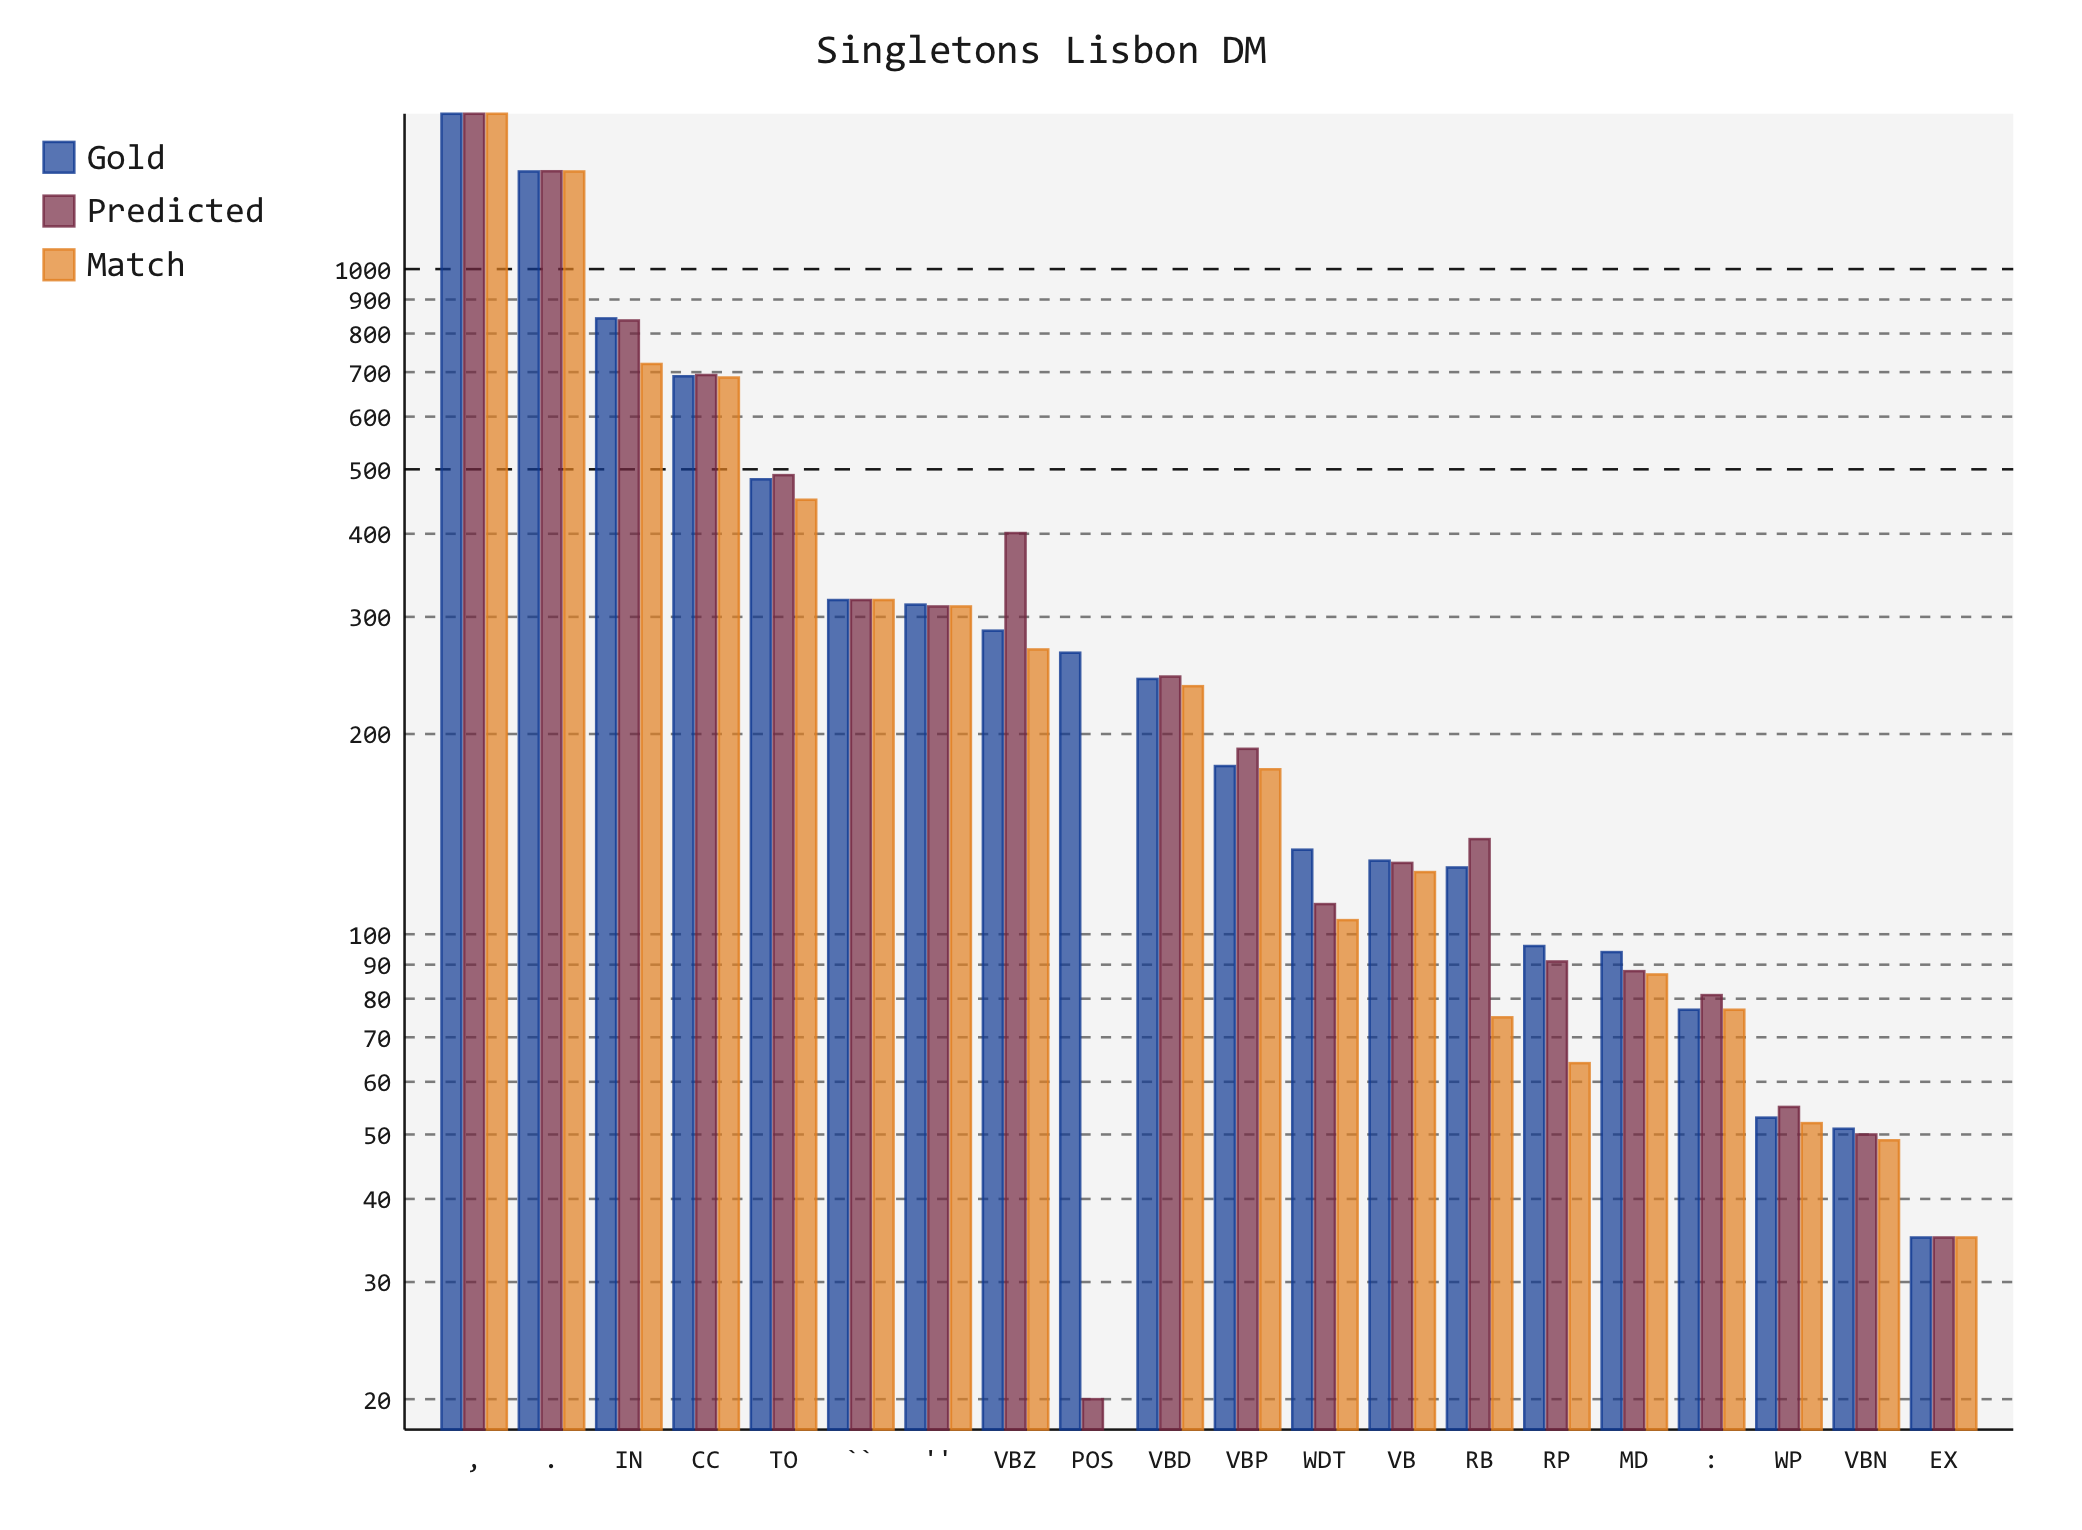
\includegraphics[width=\textwidth]{singletons_pos_DM}
    \end{minipage}\hfill
    \caption{Singletons broken down by punctuation and part-of-speech tags for the DM target representation for the Lisbon parsing system.}
    \label{fig:singletons_pos}
\end{figure}

\begin{figure}[h]
    \centering
    \begin{minipage}{0.8\textwidth}
        \centering
        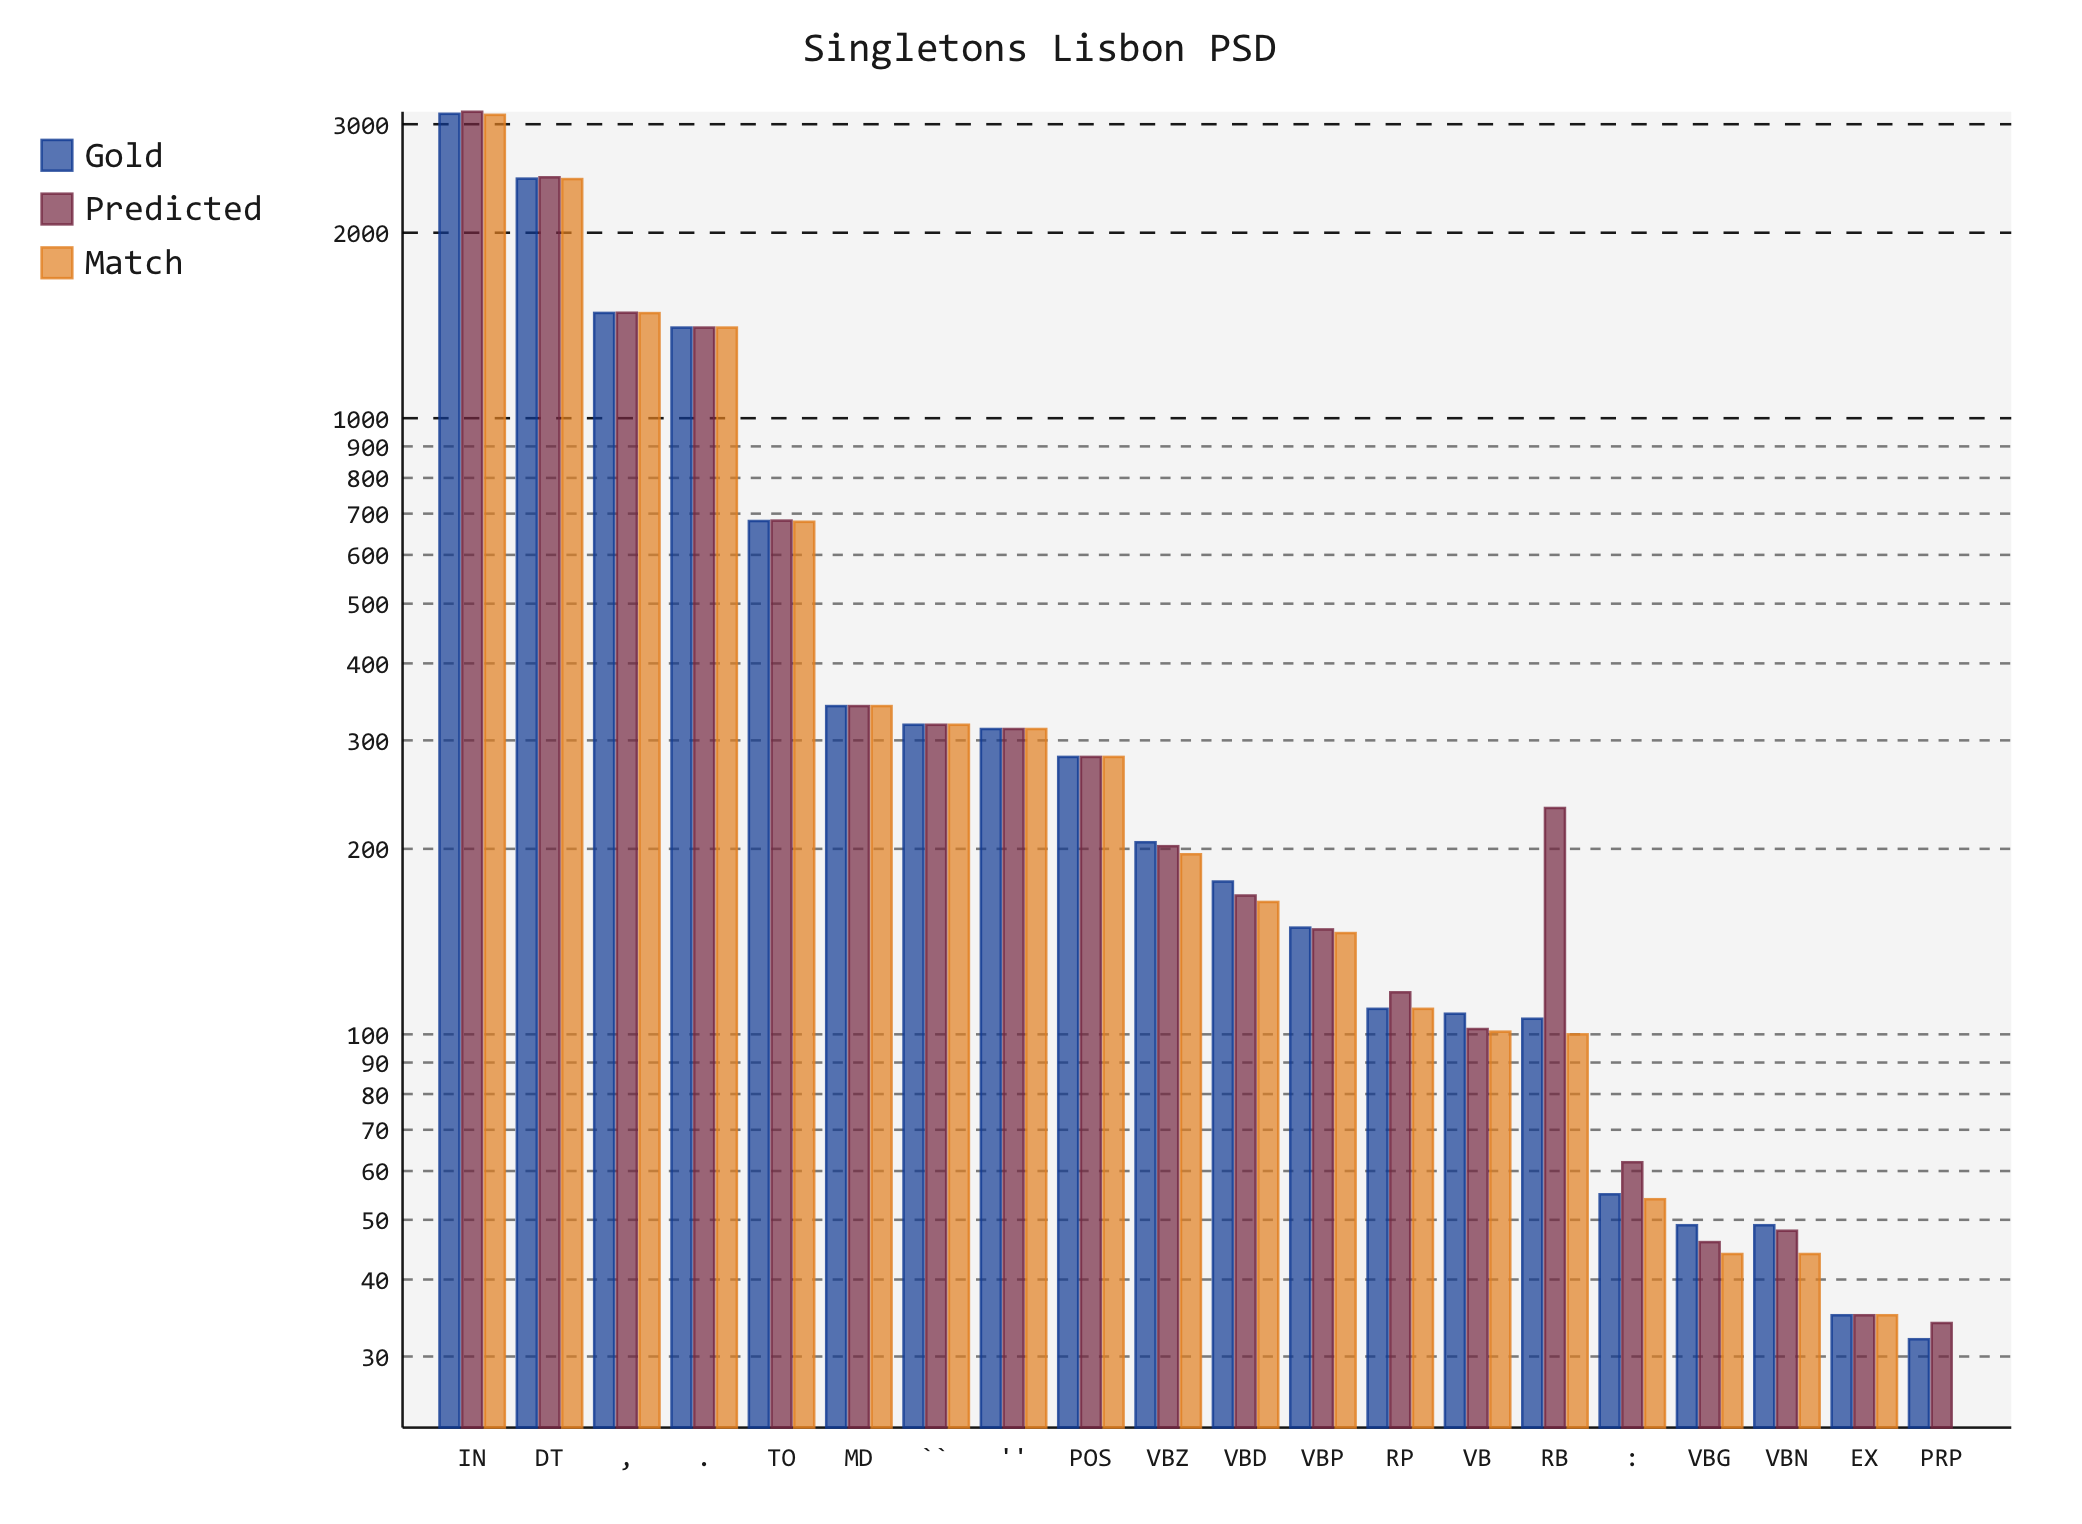
\includegraphics[width=\textwidth]{singletons_pos_PSD}
    \end{minipage}
    \caption{Singletons broken down by punctuation and part-of-speech tags for the PSD target representation for the Lisbon parsing system.}
    \label{fig:singletons_pos}
\end{figure}

Examining Table \ref{fig:singletons}, we can see the results of the three parsing systems in accurately predicting singletons. To be precise, the prediction of singletons in the three parsing systems are the result of nodes left out from the dependency structure rather than being part of a classification task. This is a step that could be considered as a binary classification task in its own right. However, the three parsing systems that are used as a basis for our analysis no not predict singletons either a step before parsing, or as a disambiguation after parsing.

Looking closer at Figure \ref{fig:singletons_pos}, we see that for the both target representation, Turku is the parser that has the highest number of singletons as the byproduct of its parsing, but a large portion of these should in fact be part of the dependency structure. The other two parsing systems also have a higher number of singletons than the gold standard. All parsing systems could therefore increase the accuracy of their parsing by attempting to parse more lexical units as part of the dependency structure.

A few cases do stand out when it comes to singletons. Again, referring to Figure \ref{fig:singletons_pos}, we see that for certain part of speech tags, the accuracy is quite dramatically different than the others. In DM this is the case for `VBZ' (verb, 3rd person singular present), `VBD' (verb, past tense), `POS' (possessive ending), `RP` (particle) and `RB' (adverb) tags. For the PSD target representation the `RB' (adverb) tag stand out. As we can see from Table \ref{fig:singletons}, the precision and recall of the Lisbon parsing system for the PSD target representation is quite higher than for DM.

\subsection{Projective and non-projective dependencies}


\section{Linguistic factors}
% part of speech
% labels

\begin{figure}[h]
    \centering
    \begin{minipage}{0.8\textwidth}
        \centering
        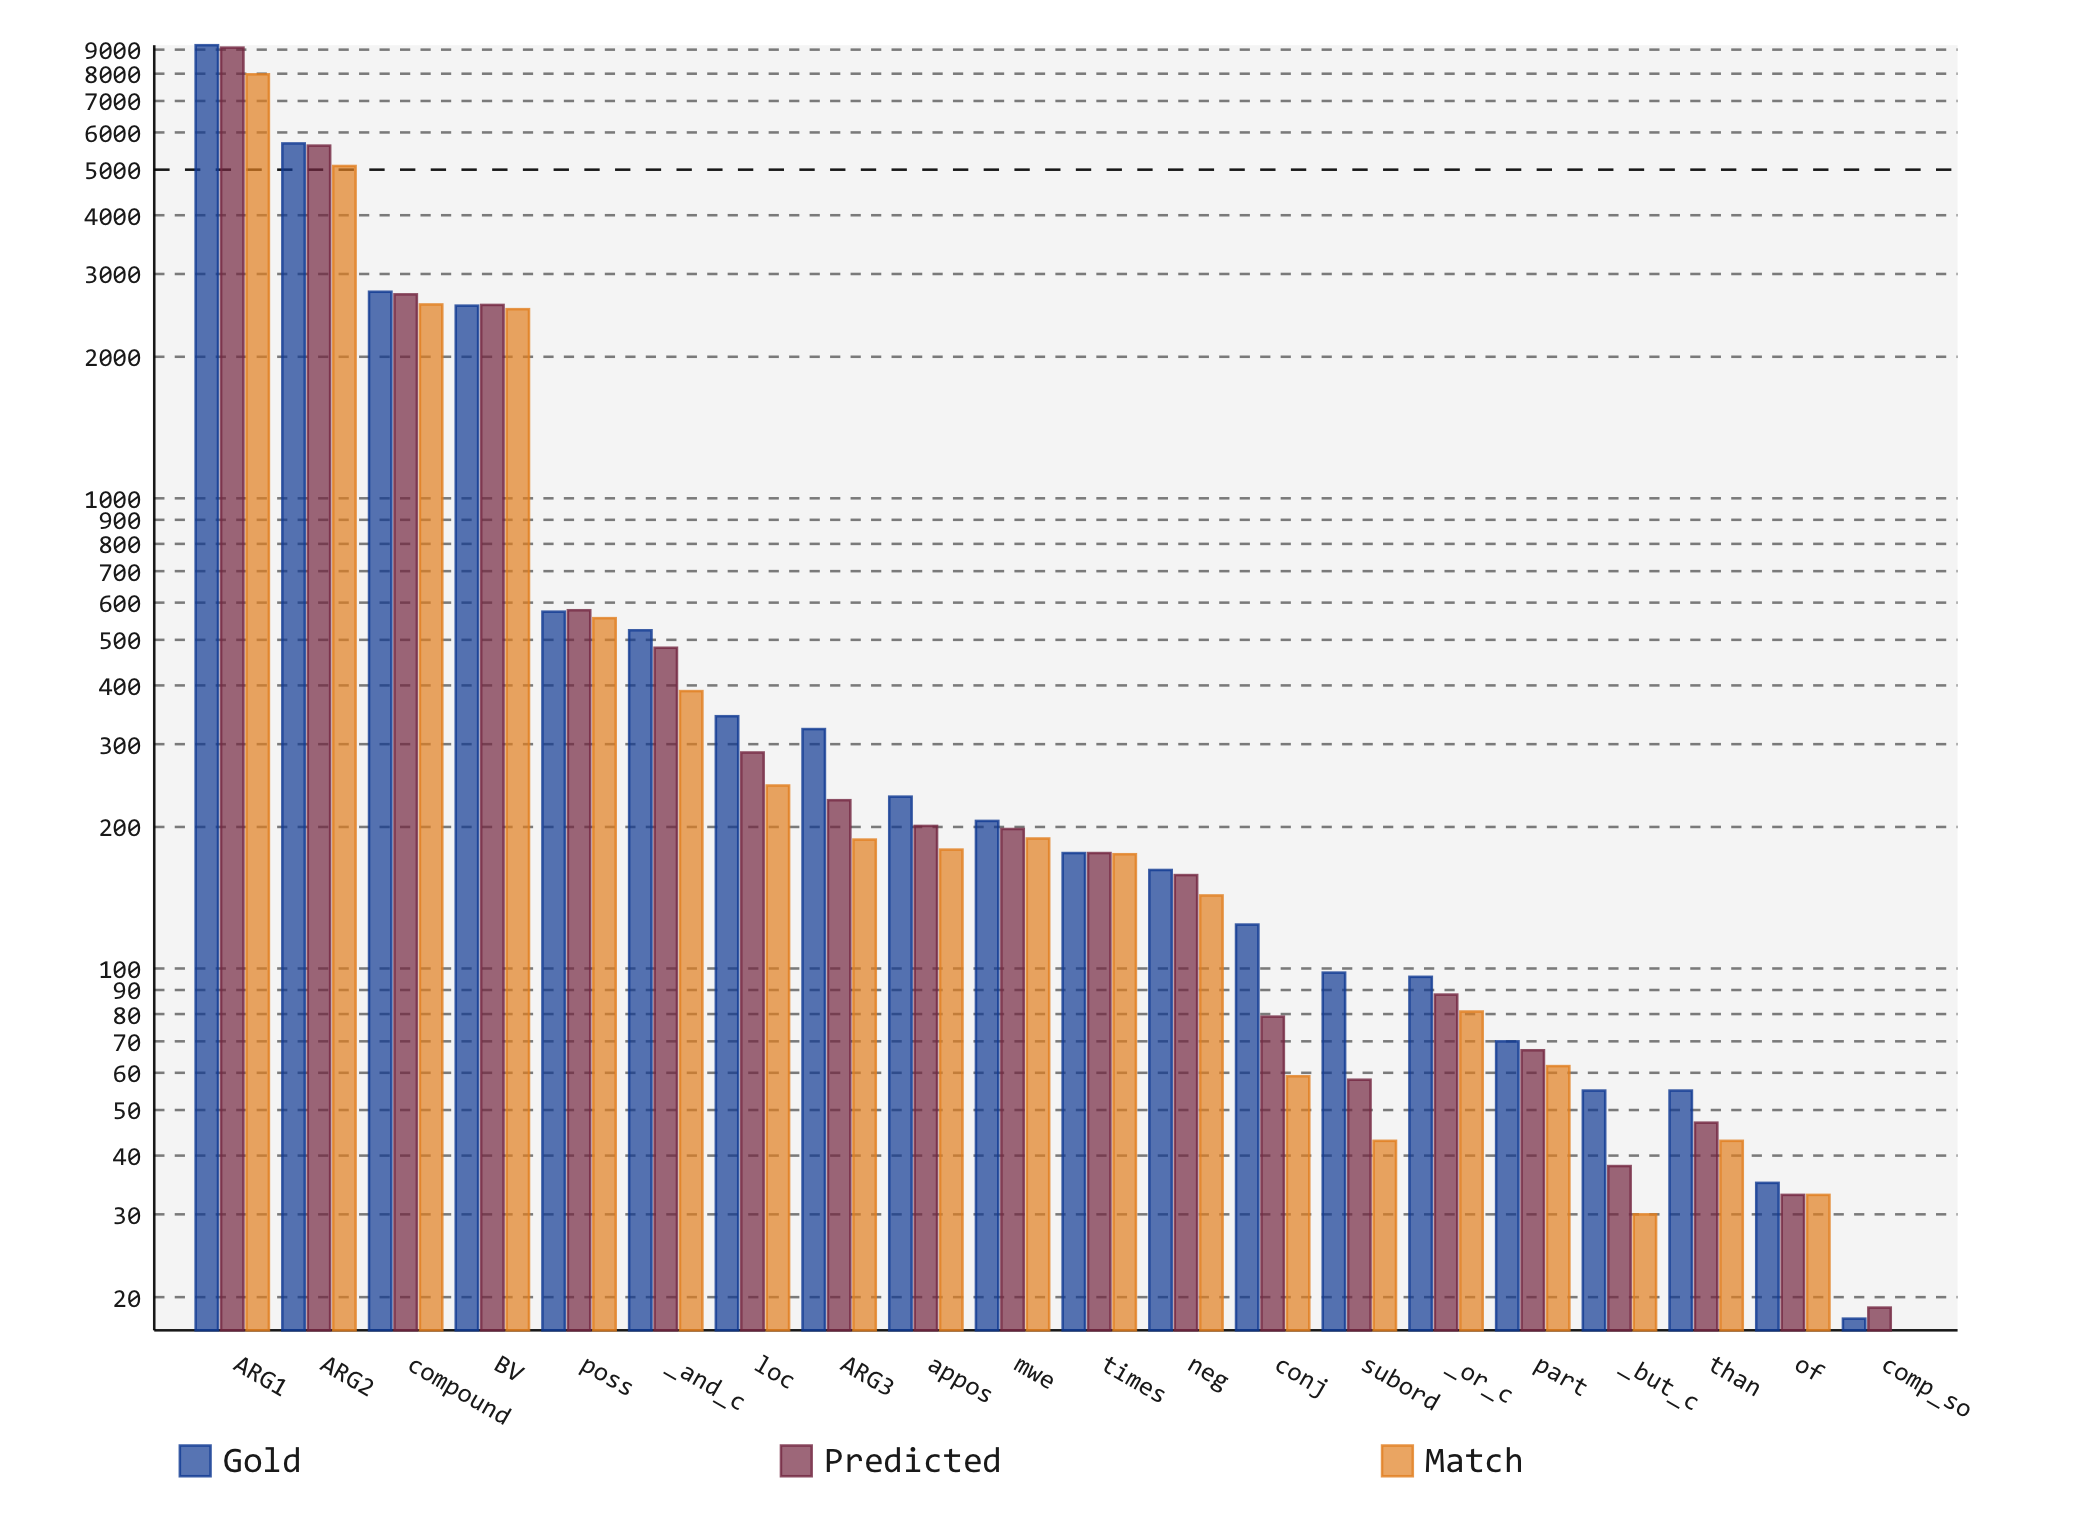
\includegraphics[width=\textwidth]{Lisbon_DM_Dep}
    \end{minipage}\hfill
    \caption{The 20 most frequent dependency types of the DM target representations. They numbers are for the frequency in gold data, the predicted data by the Lisbon parsing system, and the matches between the two.}
    \label{fig:lisbon_dep_1}
\end{figure}

\begin{figure}[h]
    \centering
    \begin{minipage}{0.8\textwidth}
        \centering
        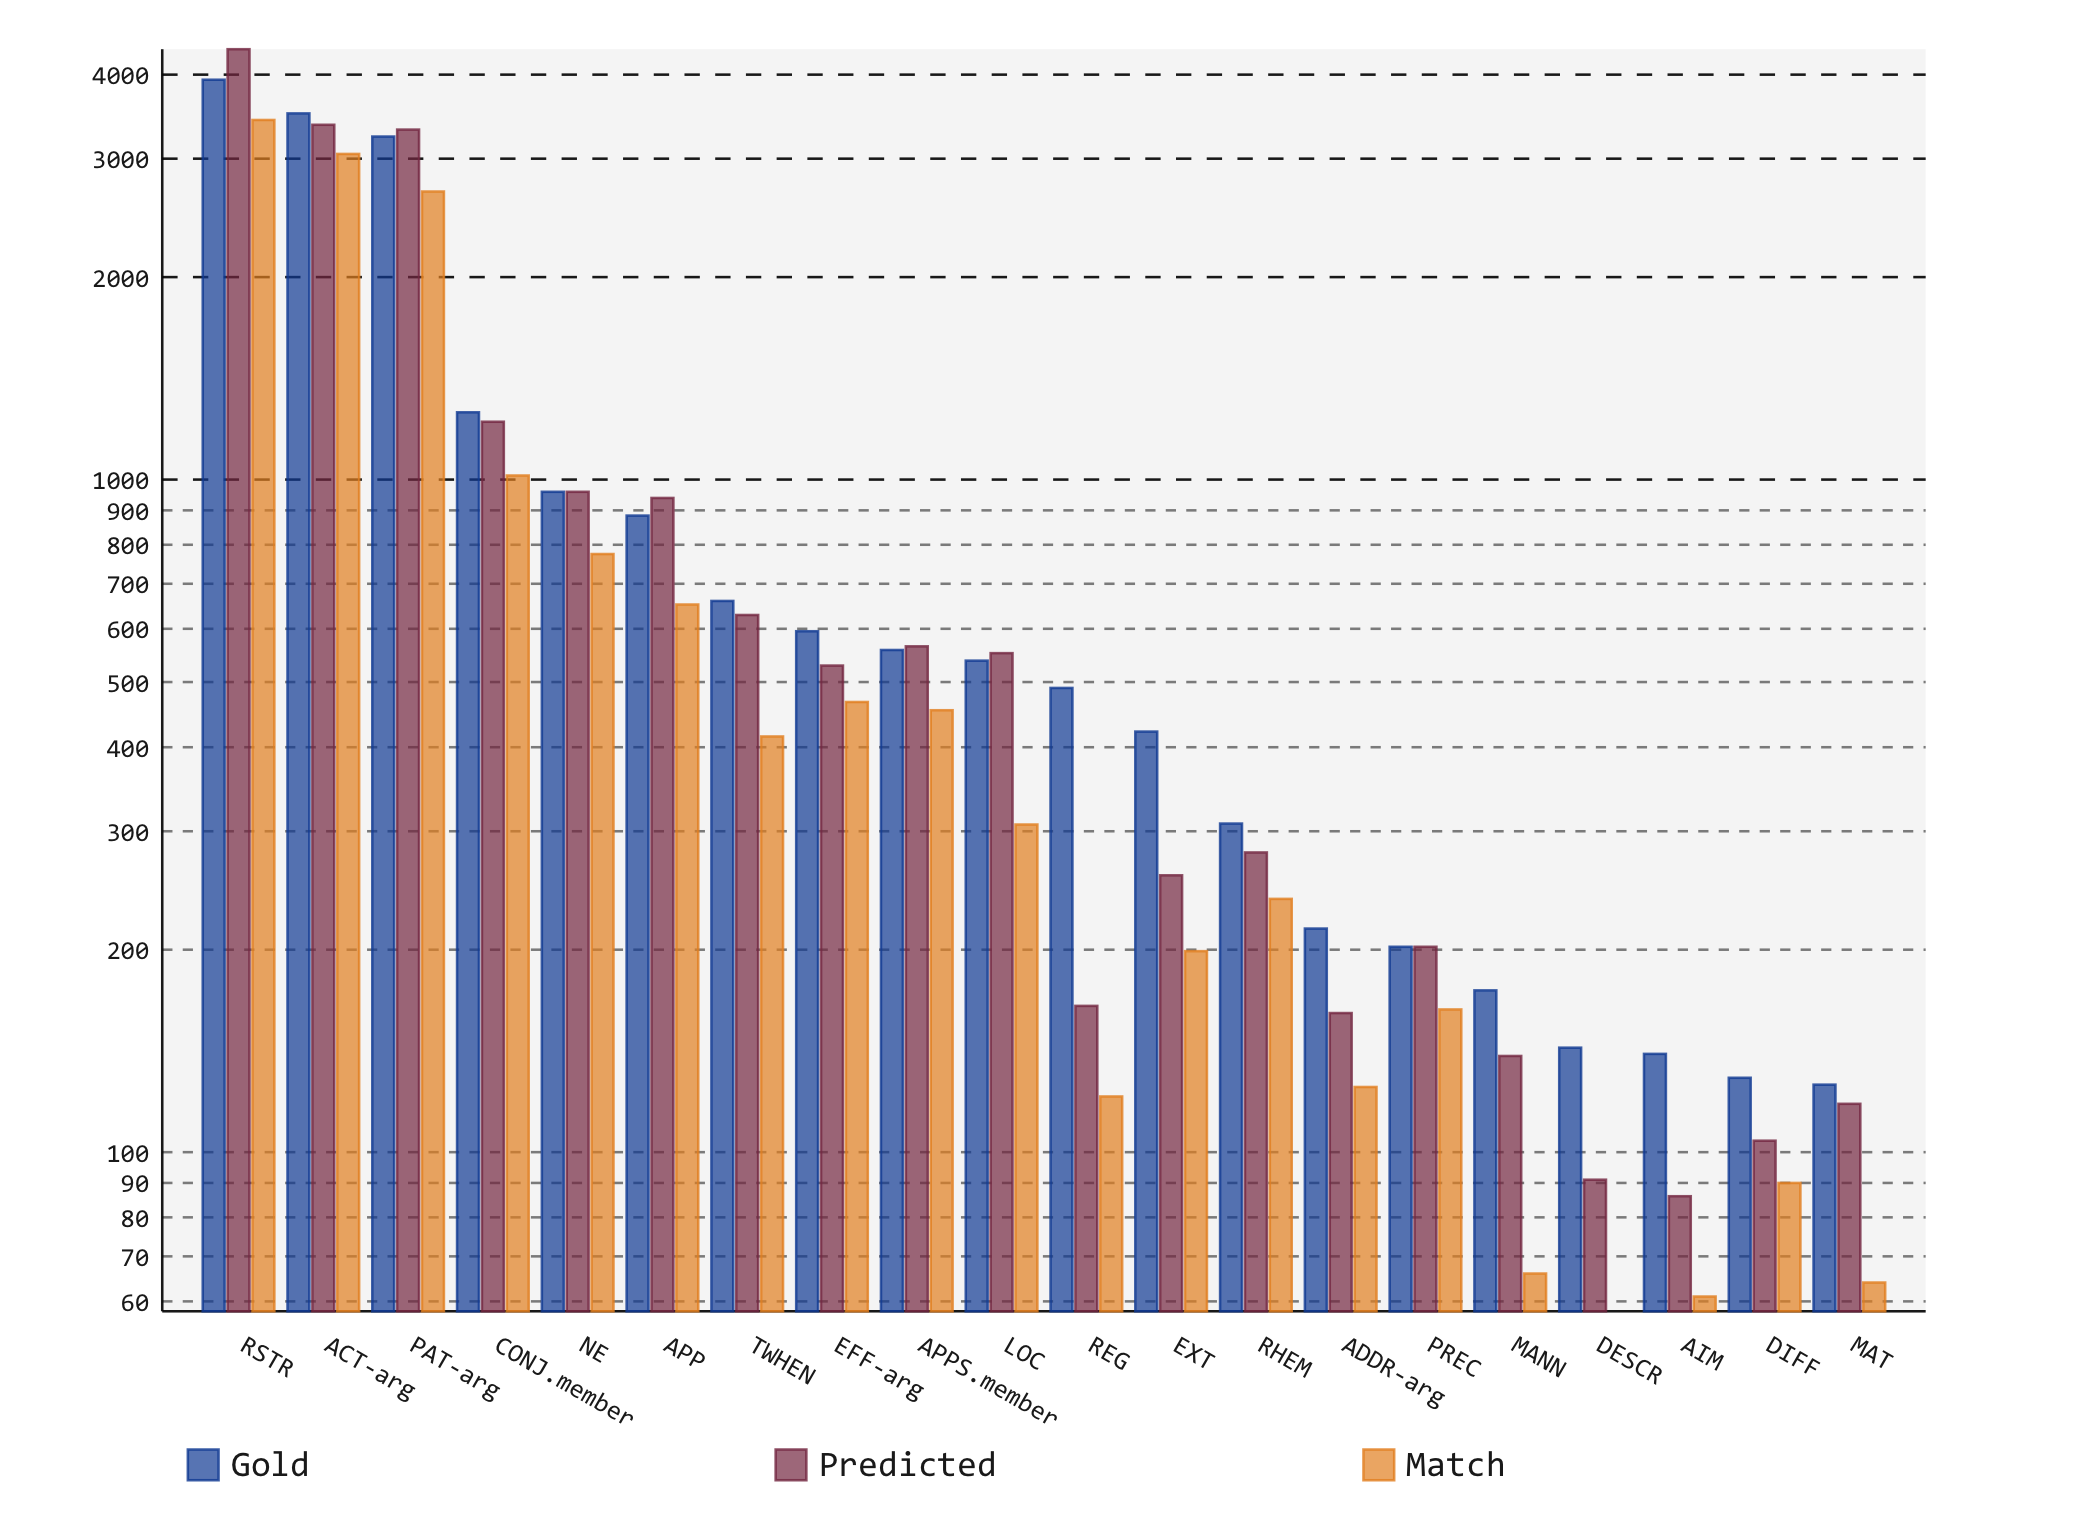
\includegraphics[width=\textwidth]{Lisbon_PSD_Dep}
    \end{minipage}
    \caption{The 20 most frequent dependency types of the PSD target representations. They numbers are for the frequency in gold data, the predicted data by the Lisbon parsing system, and the matches between the two.}
    \label{fig:lisbon_dep_2}
\end{figure}

\begin{figure}[h]
    \centering
    \begin{minipage}{0.8\textwidth}
        \centering
        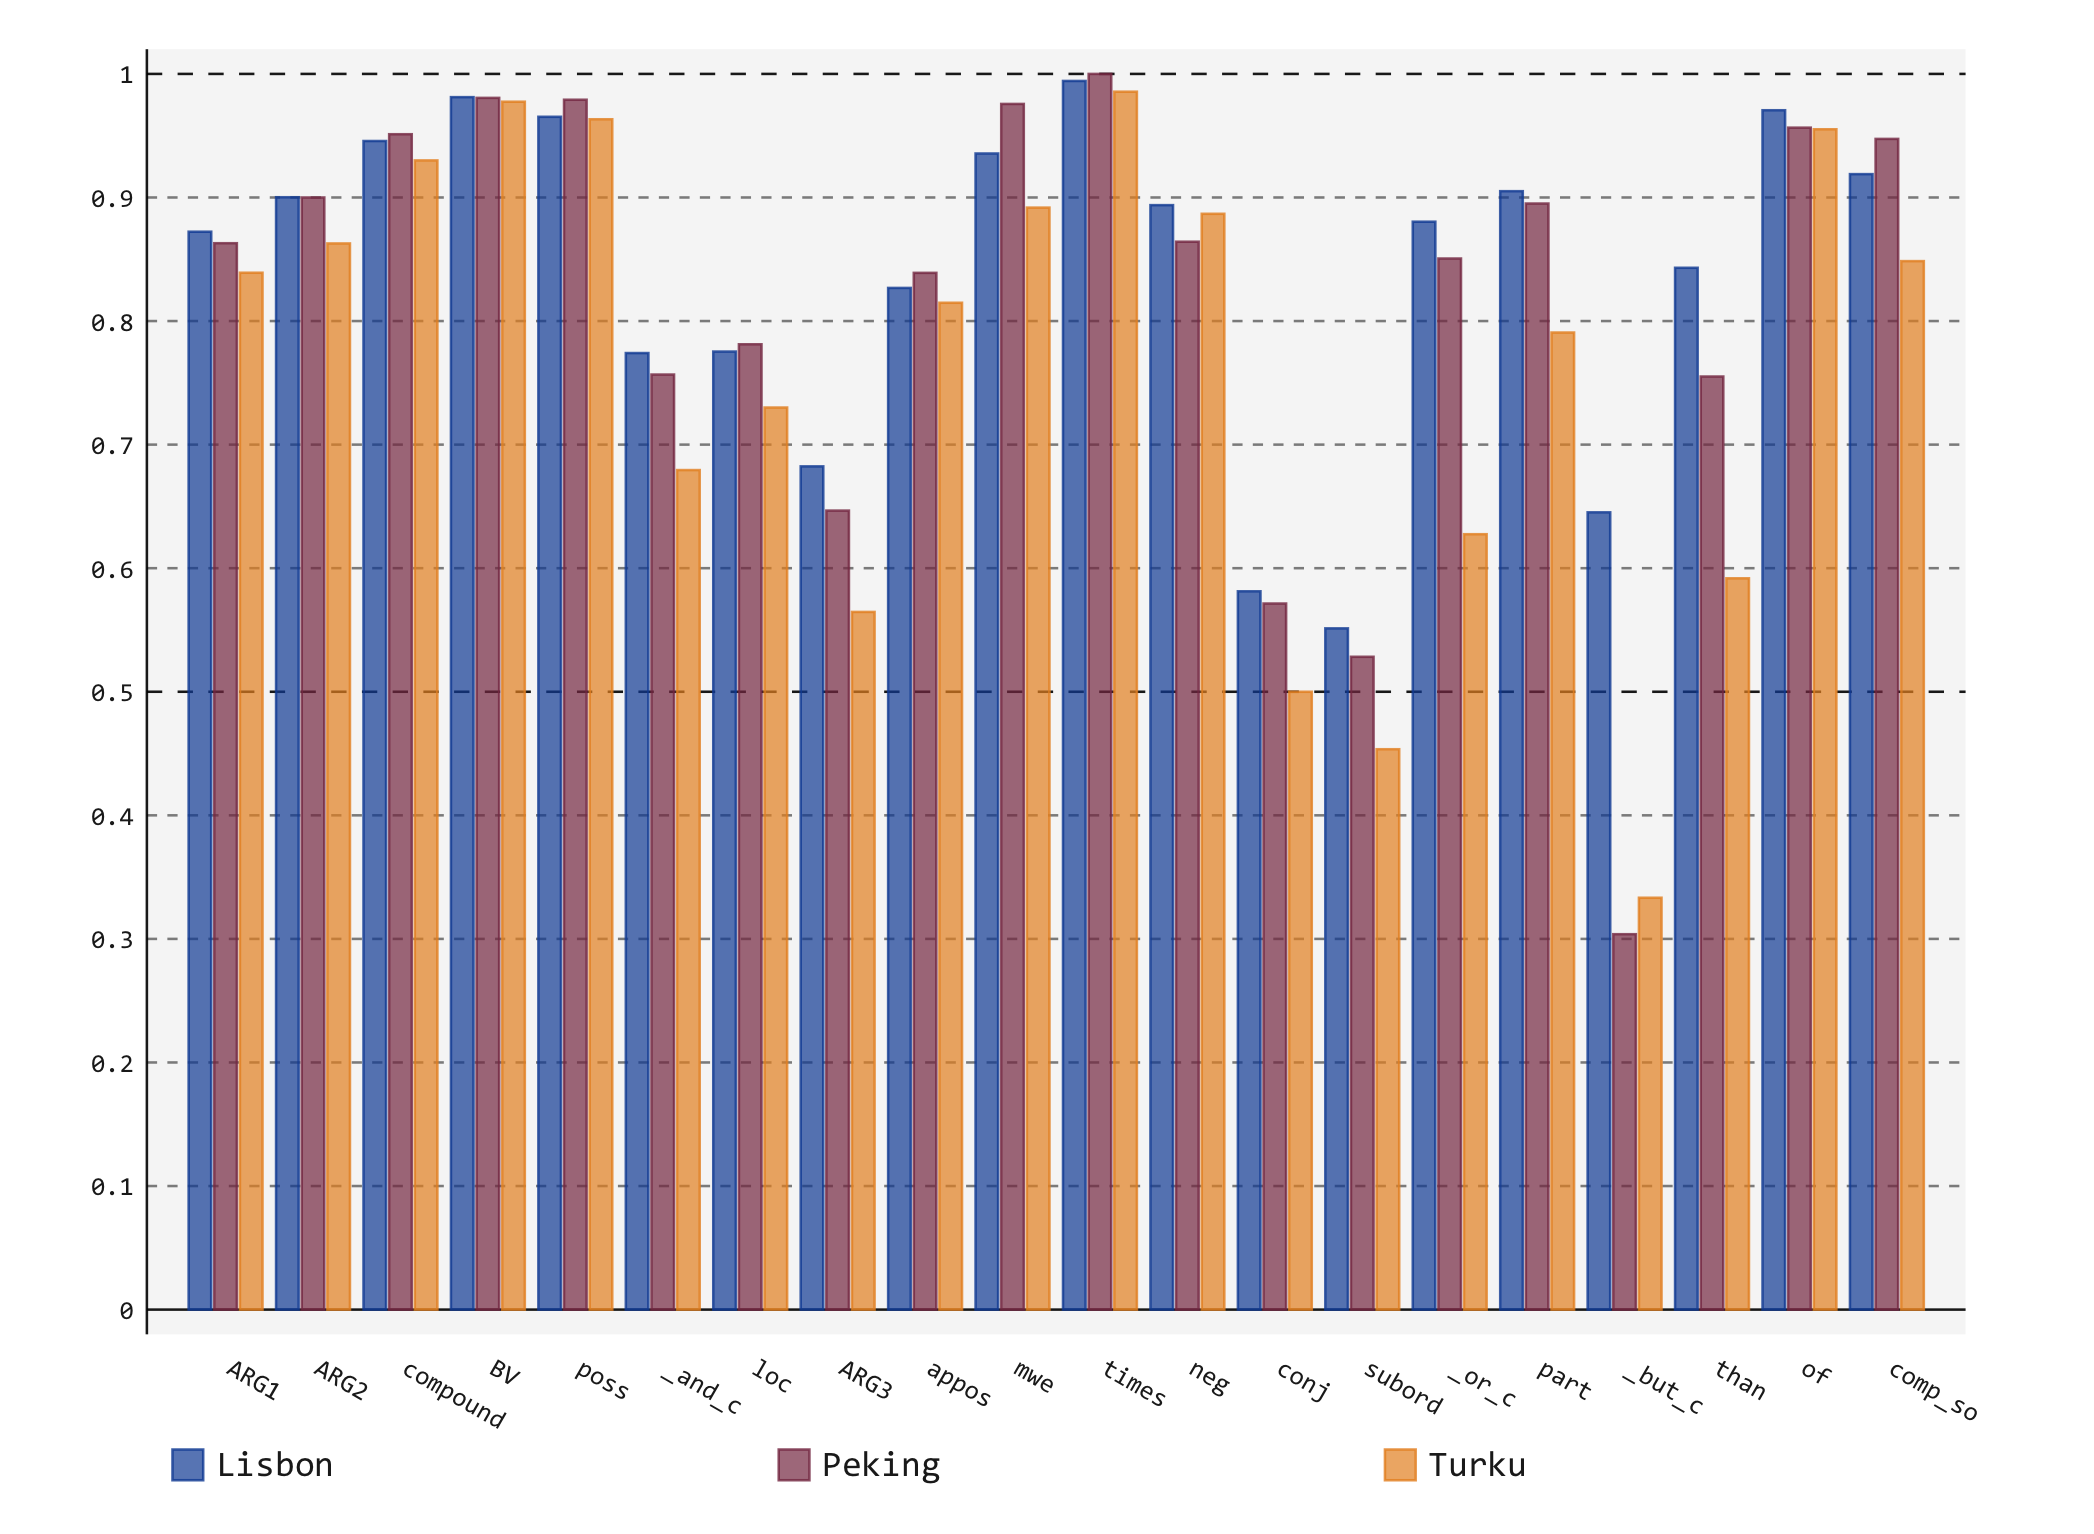
\includegraphics[width=\textwidth]{dep_dm_fscore}
    \end{minipage}\hfill
    \caption{F-score for the three parsing systems for the 20 most frequent dependency types for the DM target representations.}
    \label{fig:dep_fscore_1}
\end{figure}

\begin{figure}[h]
    \centering
    \begin{minipage}{0.8\textwidth}
        \centering
        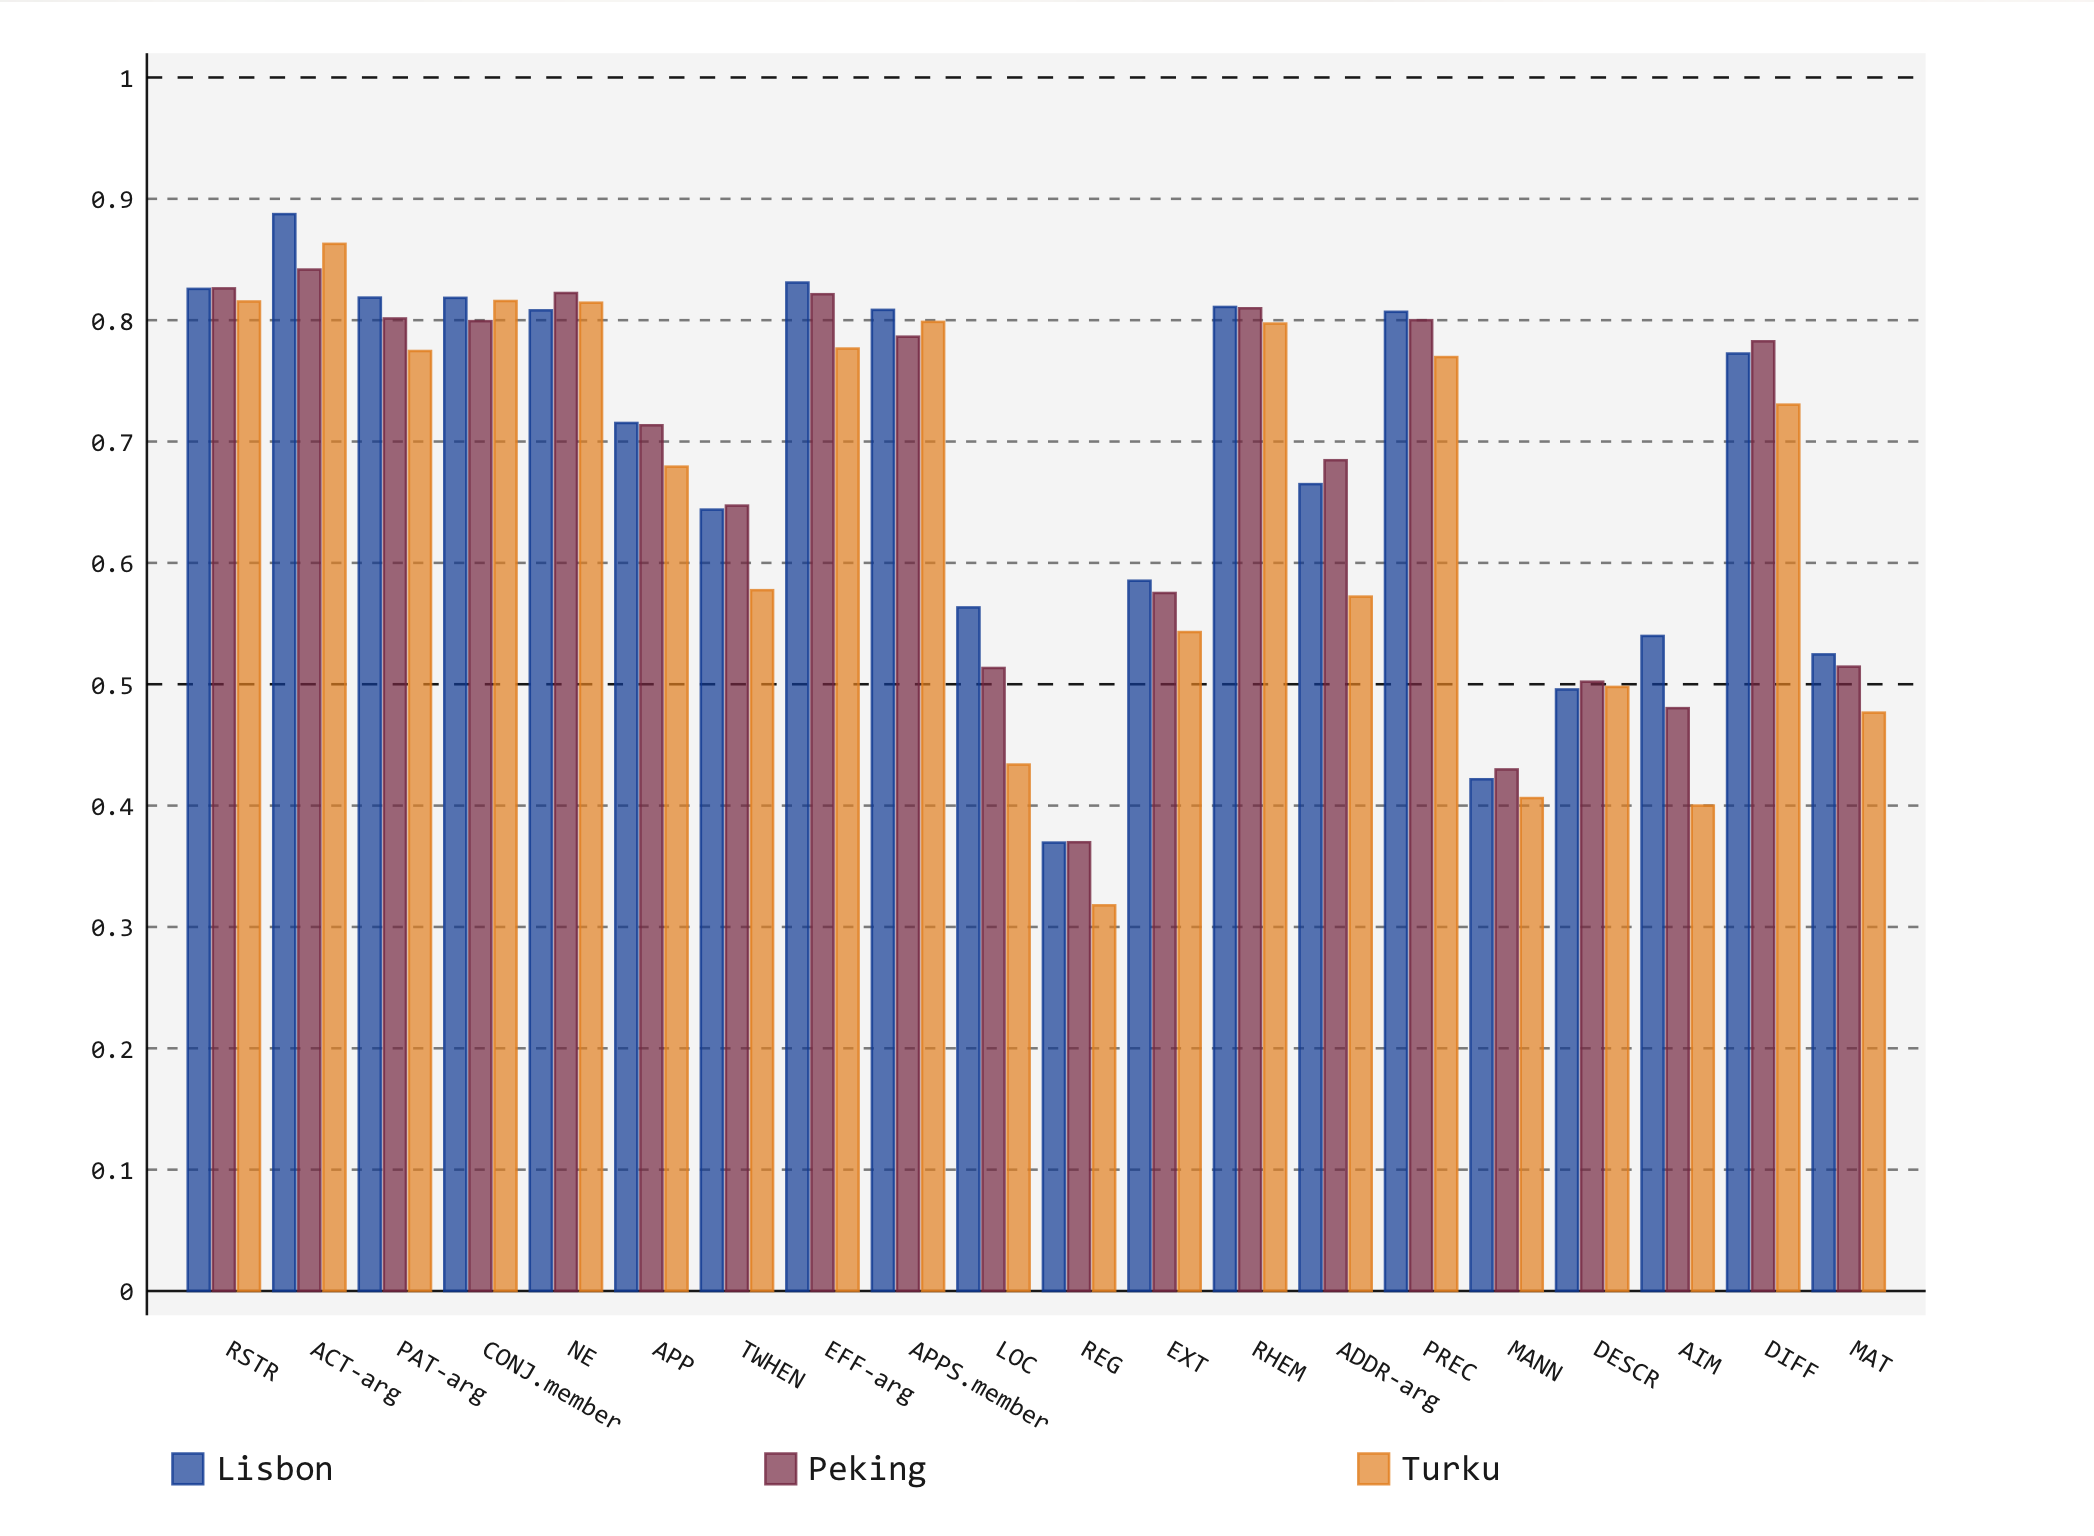
\includegraphics[width=\textwidth]{dep_psd_fscore}
    \end{minipage}
    \caption{F-score for the three parsing systems for the 20 most frequent dependency types for the PSD target representations.}
    \label{fig:dep_fscore_2}
\end{figure}

The linguistic aspects of semantic dependency parsing are some of the most interesting and insightful factors when dealing with possible errors that semantic dependency parsers can make. The factors that we will examine are (1) parts of speech and (2) dependency types. When dealing with such factors, the analysis will differ to a higher degree between the target representations than other factors. This is due to the fact that annotation schemes used in different target representations can be based on very different set of labels. It is therefore important to note that the analysis in this section may not be as general as our other findings such as the length factors.

\subsection{Parts of speech}

\subsection{Dependency types}

The dependency types found in the DM and PSD target representations follow different annotations schemes. This is true for both the number of dependencies, their distribution and what they signify. In the test data set, the DM target representation has 43 dependency types and 24813 dependencies, whereas the PSD target representation has 77 types and 22258 dependencies.

If we examine Figure \ref{fig:lisbon_dep}, we have two graphs of the 20 most frequent dependency types of both the DM and PSD target representation. The graphs present the number of dependencies in the gold data, the predictions made by the Lisbon parser, and the number of matches between the predicted and gold. We see that for the DM target representation the first two dependency types, `ARG1' and `ARG2', account for 14884 of the 24813 dependencies, while for the PSD target representation the distribution is more evenly spreak across the most frequent types. In terms of the parsing accuracy, we see that the number of gold and predicte are more similar for DM than for PSD, where there are more fluctuations.



\section{Frames}
% just frames
% complete frames

\section{Conclusions}

In this chapter we have examined the results of Peking, Turku and Lisbon parsing systems as submitted to SemEval-2015. Our examinations have uncovered some interesting phenomena, such as the fact that the overall accuracy of all parsing systems drop in correlation to sentence and dependency length. That the parsing systems are more prone to errors in regards to certain graph and linguistic factors. We have shown that, although some parsing errors can be attributed to lower frequency in the training data, there are also other factors that impact parsing where an increase in training data would not necessarily translate to better results. These type of errors are more related to the technical aspects of the parsing systems themselves. We have seen that different parsing systems produce different types of errors. The results of such an overall analysis could lead the way for ensemble methods where an error analysis is used as basis for weighting.

However, the error analysis did not produce enough evidence to build an overall strategy for improving upon the results of the three semantic dependency parsers examined in this chapter. As mentioned previously, we have instead chosen to focus on improving the accuracy of the classification task of predicting semantic frames. This aspect of semantic dependency parsing is not well researched, and the results of our analysis seem to indicate that there can be room for improvement. In the next chapter we present a set of experiments where we attempt to improve upon the results of SemEval-2015.

% Input for graph images
% \begin{figure}[h]
% \caption{Caption}
% \centering
% 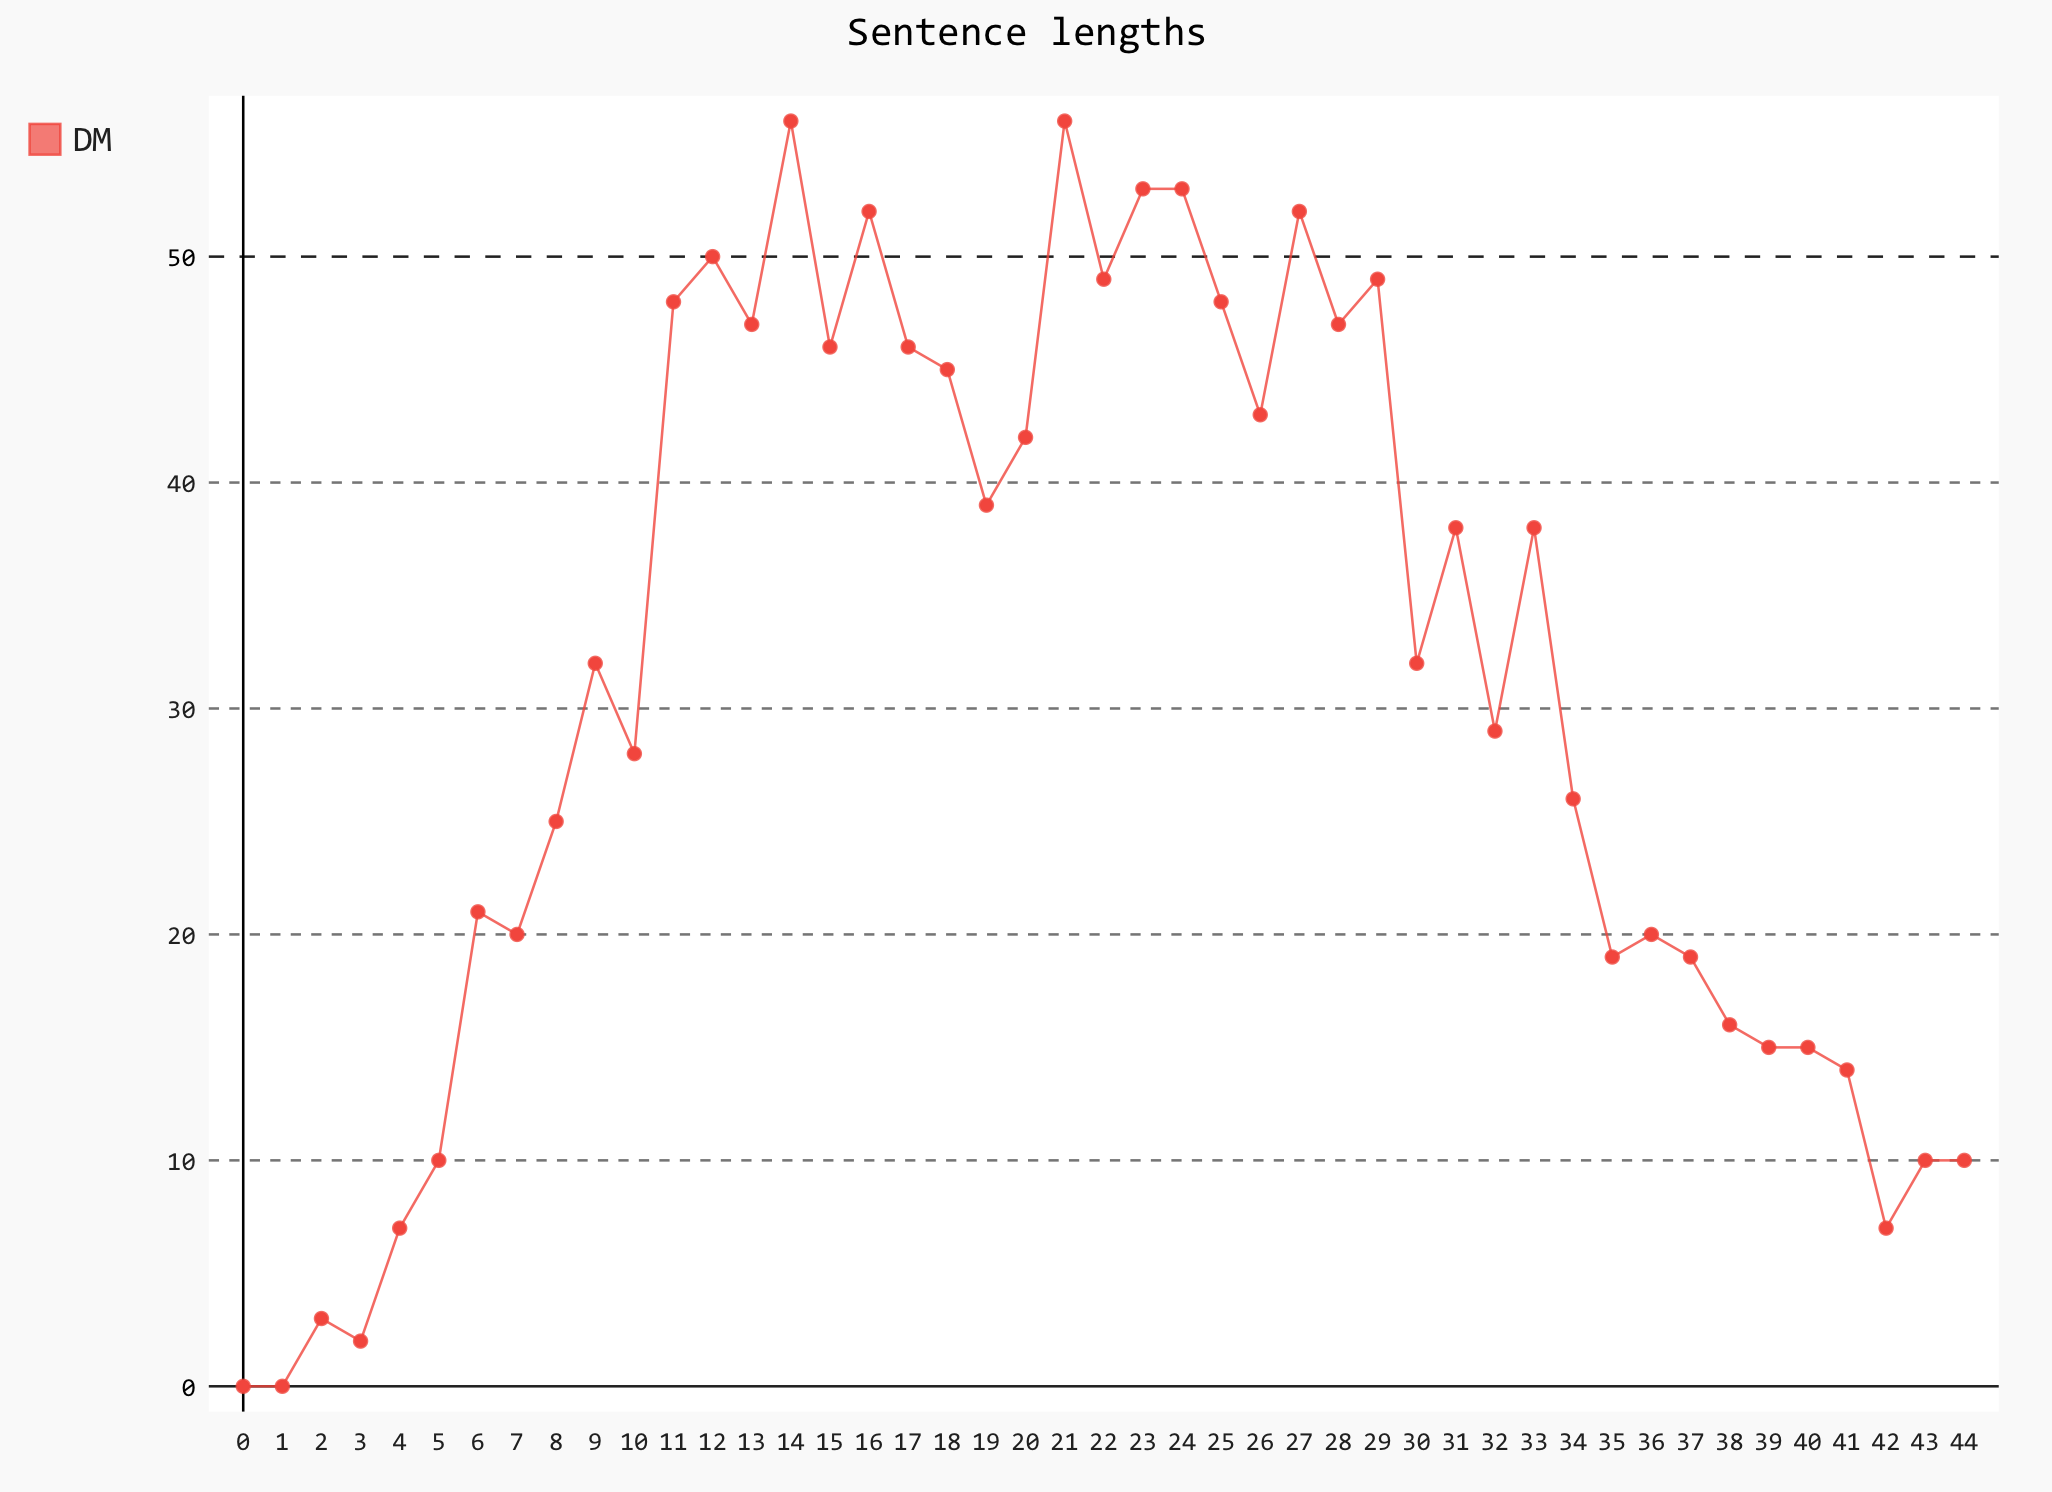
\includegraphics[width=\textwidth]{sentence_length}
% \label{fig:sentence_length}
% \end{figure}